%! Author = crist
%! Date = 25/10/2026

\spacing{1.3}
%----------------------------------------------------------------------------------------
%	UNIDAD 9: EL MOVIMIENTO CIRCULAR. LA GRAVEDAD Y OTRAS FUERZAS (4.º ESO)
%   Figuras: images/UD9/*.pdf (fuente HTML en images/UD9/html, SVG en images/UD9/svg)
%   Gráficas con pgfplots: estilo «grafica», definido al inicio de la UD7.
%   Datos usados en toda la unidad: G = 6,67·10^-11 N·m²/kg², M_T = 5,97·10^24 kg, R_T = 6,37·10^6 m.
%----------------------------------------------------------------------------------------

% Mapa conceptual del tema (fuente en images/mapas_conceptuales/html/temas.js)
\begin{figure}[H]
    \centering
    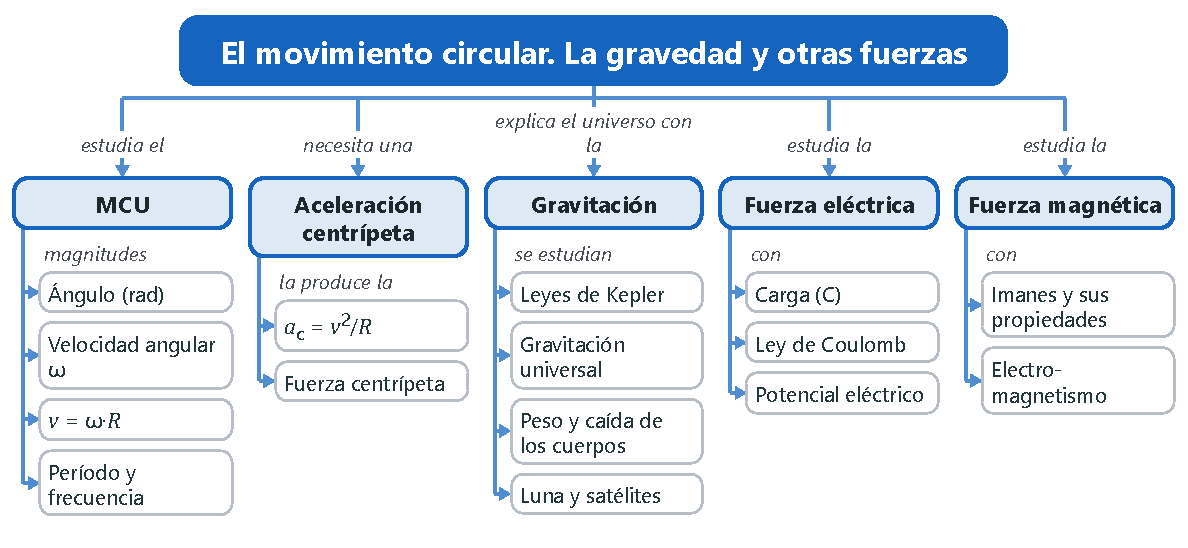
\includegraphics[width=\textwidth]{images/mapas_conceptuales/mapa_UD9}
\end{figure}

%========================================================================================
%\section*{Para empezar: los satélites meteorológicos}
%\addcontentsline{toc}{section}{Para empezar: los satélites meteorológicos}
%========================================================================================
%
%Los \textbf{satélites meteorológicos} envían sin parar datos sobre el estado de la atmósfera en grandes zonas del planeta, y los servicios de predicción del tiempo dependen de esas imágenes.
%
%Los satélites \textbf{Meteosat} de la Agencia Espacial Europea (ESA) son \textbf{geoestacionarios}: giran al mismo ritmo que la Tierra y siempre «miran» la misma zona de la superficie, de la que toman una imagen cada media hora (salvo las regiones polares, que ven mal). Los satélites de \textbf{órbita polar}, en cambio, vuelan mucho más bajos, a unos \qty{800}{\km} de altura, y trabajan por parejas para que sus datos nunca tengan más de seis horas de retraso. Entre todos hacen más de \num{16000} mediciones al día y recorren el planeta entero en 24 horas.
%
%Saber con antelación qué tiempo va a hacer permite tomar medidas: preparar a la población ante un temporal, planificar las cosechas o hacer más segura la navegación. Por eso estos satélites tienen que ver con el \textbf{ODS 11} (\emph{Ciudades y comunidades sostenibles}) y el \textbf{ODS 13} (\emph{Acción por el clima}).
%
%¿Por qué un satélite se mantiene en órbita sin caer? ¿Por qué tarda más en dar una vuelta cuanto más lejos está? En esta unidad lo vamos a entender: estudiaremos el movimiento circular, la fuerza que lo produce y la gravedad, la fuerza que mantiene unidos la Luna, los planetas y los satélites. Terminaremos con otras dos fuerzas de la naturaleza: la eléctrica y la magnética.
%
%\begin{exercise}
%    ¿Para qué sirven los satélites meteorológicos? ¿Son útiles solo para predecir el tiempo de grandes zonas o también a escala local?
%    \begin{solu}
%        Proporcionan \textcolor{red}{datos actualizados continuamente} de las condiciones meteorológicas de grandes zonas. Son imprescindibles tanto para la predicción \textcolor{red}{local como para la de grandes zonas}, porque los modelos de predicción se alimentan de sus imágenes.
%    \end{solu}
%\end{exercise}
%
%\begin{exercise}
%    ¿En qué dos tipos de órbita trabajan los satélites meteorológicos? ¿Qué significa que los Meteosat sean geoestacionarios?
%    \begin{solu}
%        En \textcolor{red}{órbitas geoestacionarias} y en \textcolor{red}{órbitas polares}. Un satélite geoestacionario tarda lo mismo que la Tierra en dar una vuelta (24 horas), por lo que \textcolor{red}{permanece siempre sobre la misma zona} de la superficie.
%    \end{solu}
%\end{exercise}
%
%\begin{exercise}
%    ¿A qué altura vuelan los satélites de órbita polar? ¿Por qué actúan por parejas?
%    \begin{solu}
%        A unos \textcolor{red}{\qty{800}{\km}} de altura. Trabajan por parejas para que los datos que captan \textcolor{red}{no tengan más de seis horas de retraso}.
%    \end{solu}
%\end{exercise}
%
%\begin{exercise}
%    Un satélite no puede evitar un temporal. ¿Por qué, entonces, se relaciona con los ODS 11 y 13? Debatidlo en clase.
%    \begin{solu}
%        Respuesta libre. Anticipar el tiempo permite \textcolor{red}{tomar medidas preventivas} ante temporales, inundaciones u olas de calor, proteger a la población de las ciudades (ODS 11) y adaptarse a los efectos del cambio climático (ODS 13).
%    \end{solu}
%\end{exercise}

%========================================================================================
\section[Características del movimiento circular uniforme]{¿Cuáles son las características del movimiento circular uniforme?}
%========================================================================================

El extremo de la aguja de los minutos de un reloj da una vuelta completa cada hora. Su rapidez es siempre la misma, pero la dirección en la que se mueve cambia en cada instante. Es un ejemplo de movimiento circular uniforme.

\begin{definition}[Movimiento circular uniforme (MCU)]
    Es el movimiento de un cuerpo cuya trayectoria es una \textbf{circunferencia} y que recorre \textbf{arcos iguales en tiempos iguales}.
\end{definition}

El MCU se podría describir con las magnitudes de los movimientos rectilíneos (posición sobre la trayectoria, velocidad\ldots), pero es mucho más sencillo hacerlo con \textbf{magnitudes angulares}.

\begin{figure}[H]
    \centering
    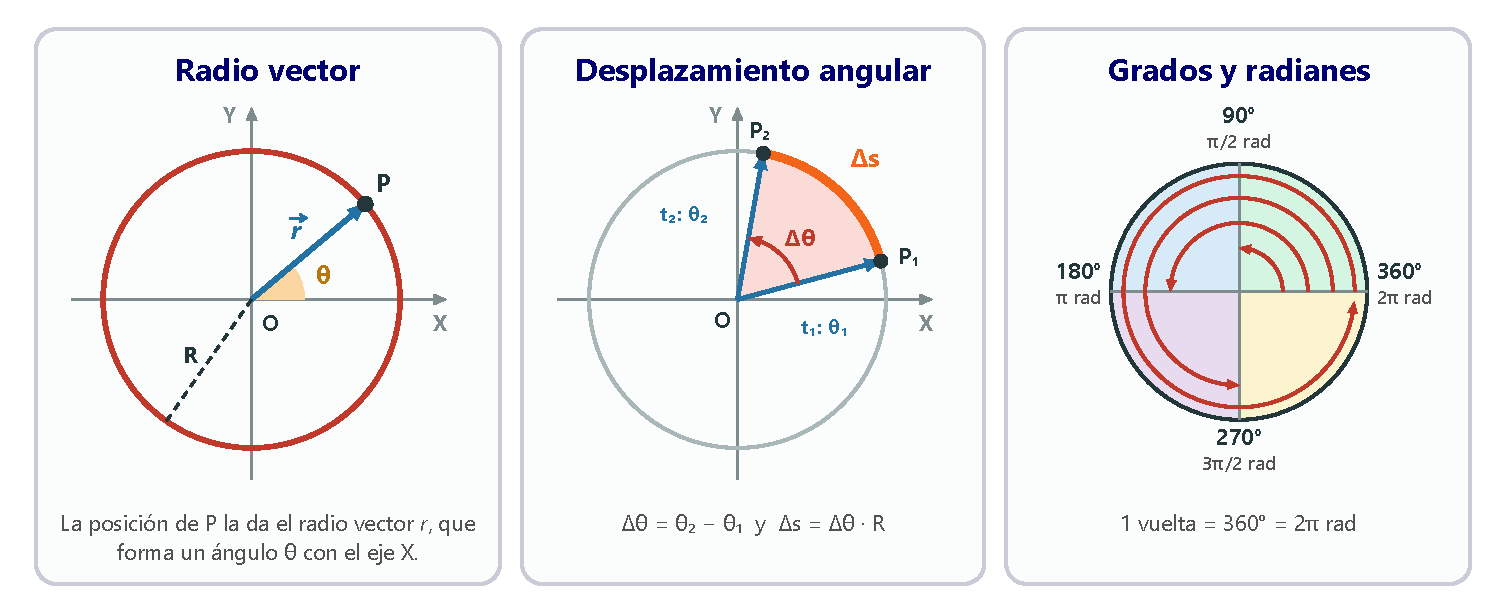
\includegraphics[width=\textwidth]{images/UD9/mcu_magnitudes}
    \caption{Radio vector, desplazamiento angular y medida de ángulos en grados y radianes.}
    \label{fig:mcu_magnitudes}
\end{figure}

\subsection{¿Cómo se indica la posición de un punto? El radio vector}

En un MCU, la posición de un punto P se da con el \textbf{radio vector}, \(\vec{r}\), que tiene su origen en el centro de la circunferencia, O, y su extremo en P (figura~\ref{fig:mcu_magnitudes}). Su módulo es el radio de la circunferencia, \(R\), y forma un ángulo \(\theta\) con el eje X.

\subsection{¿Cómo se mide el cambio de posición? El desplazamiento angular}

Si en el instante \(t_1\) el radio vector forma un ángulo \(\theta_1\) con el eje X y en el instante \(t_2\) forma un ángulo \(\theta_2\), el \textbf{desplazamiento angular} es el ángulo que ha barrido:
\[ \Delta\theta = \theta_2 - \theta_1 \]
Mientras tanto, el punto ha recorrido sobre la circunferencia un arco \(\Delta s\). Las tres magnitudes se relacionan así:
\[ \text{desplazamiento angular} = \frac{\text{arco}}{\text{radio}} \qquad\Rightarrow\qquad \Delta\theta = \frac{\Delta s}{R} \]

\paragraph{¿En qué unidades se mide el desplazamiento angular? El radián.} Un ángulo se puede medir en \textbf{grados} (una circunferencia tiene \ang{360}), en \textbf{revoluciones} o vueltas (una circunferencia es una vuelta) o en \textbf{radianes}, que es la unidad del SI.

\begin{definition}[Radián]
    Un \textbf{radián} (\unit{\radian}) es el ángulo que abarca un arco de longitud igual al radio. Como la longitud de la circunferencia es \(2\pi R\), una vuelta completa son \(2\pi\) radianes:
    \[ 1~\text{vuelta} = \ang{360} = 2\pi~\unit{\radian} \qquad\qquad 1~\unit{\radian} \approx \ang{57.3} \]
\end{definition}

\subsection{¿Qué es la velocidad angular?}

\begin{definition}[Velocidad angular]
    La \textbf{velocidad angular}, \(\omega\), es el ángulo barrido por el radio vector por unidad de tiempo:
    \[ \omega = \frac{\Delta\theta}{\Delta t} \]
    En el MCU es \textbf{constante}. Su ecuación de dimensiones es \([\omega] = \mathrm{T}^{-1}\).
\end{definition}

Además del radián por segundo (\unit{\radian\per\s}), que es la unidad del SI, se usan las \textbf{revoluciones por minuto} (rpm) y las \textbf{revoluciones por segundo} (rps):
\[ 1~\text{rpm} = \frac{1~\text{vuelta}}{1~\text{min}} = \frac{2\pi~\unit{\radian}}{\qty{60}{\s}} = \frac{\pi}{30}~\unit{\radian\per\s} \qquad\qquad 1~\text{rps} = \frac{1~\text{vuelta}}{1~\unit{\s}} = 2\pi~\unit{\radian\per\s} \]

\subsection{Ecuación del MCU}

Como la velocidad angular es constante, el ángulo barrido es proporcional al tiempo:
\[ \Delta\theta = \omega \cdot \Delta t \qquad\Rightarrow\qquad \theta = \theta_0 + \omega \cdot t \]
Si en el instante inicial el ángulo es cero (\(\theta_0 = 0\)), la ecuación queda \(\theta = \omega \cdot t\). Fíjate en que se parece mucho a la ecuación del MRU, \(x = x_0 + v \cdot t\).

\begin{example}
    Un móvil describe un MCU con una velocidad angular de \qty{6}{\radian\per\s}. Calcula el ángulo que barre en \qty{10}{\s} y el tiempo que tarda en dar una vuelta.

    \(\theta = \omega \cdot t = \qty{6}{\radian\per\s} \cdot \qty{10}{\s} = \textcolor{red}{\qty{60}{\radian}}\) (casi diez vueltas). Una vuelta son \(2\pi\) rad, así que:
    \[ t = \frac{\theta}{\omega} = \frac{2\pi~\unit{\radian}}{\qty{6}{\radian\per\s}} = \frac{\pi}{3}~\unit{\s} = \textcolor{red}{\qty{1.05}{\s}} \]
\end{example}

\begin{exercise}
    ¿A cuántos grados equivalen \(\pi\), \(\pi/2\), \(\pi/3\) y \(\pi/4\) radianes? ¿A cuántos radianes equivalen dos vueltas?
    \begin{solu}
        Como \(\pi~\unit{\radian} = \ang{180}\): \(\pi~\unit{\radian} = \textcolor{red}{\ang{180}}\); \(\pi/2 = \textcolor{red}{\ang{90}}\); \(\pi/3 = \textcolor{red}{\ang{60}}\); \(\pi/4 = \textcolor{red}{\ang{45}}\). Dos vueltas son \(2 \cdot 2\pi = \textcolor{red}{4\pi~\unit{\radian}}\).
    \end{solu}
\end{exercise}

\begin{exercise}
    Calcula la velocidad angular de las agujas de las horas, de los minutos y de los segundos de un reloj.
    \begin{solu}
        Cada aguja da una vuelta (\(2\pi\) rad) en 12 h, 1 h y 1 min, respectivamente:
        \[ \omega_h = \frac{2\pi}{\qty{43200}{\s}} = \textcolor{red}{\qty{1.45e-4}{\radian\per\s}} \qquad \omega_{min} = \frac{2\pi}{\qty{3600}{\s}} = \textcolor{red}{\qty{1.75e-3}{\radian\per\s}} \]
        \[ \omega_s = \frac{2\pi}{\qty{60}{\s}} = \textcolor{red}{\qty{0.105}{\radian\per\s}} \]
    \end{solu}
\end{exercise}

\begin{exercise}
    Expresa en radianes por segundo estas velocidades angulares: \num{1.5} rps, 1 rpm, 60 rps y 30 rpm.
    \begin{solu}
        \(\num{1.5}~\text{rps} = \num{1.5} \cdot 2\pi = \textcolor{red}{3\pi~\unit{\radian\per\s}}\); \(1~\text{rpm} = \textcolor{red}{\pi/30~\unit{\radian\per\s}}\); \(60~\text{rps} = \textcolor{red}{120\pi~\unit{\radian\per\s}}\); \(30~\text{rpm} = 30 \cdot \pi/30 = \textcolor{red}{\pi~\unit{\radian\per\s}}\).
    \end{solu}
\end{exercise}

\subsection{¿Qué relación hay entre las magnitudes lineales y las angulares?}

Ya sabemos que \(\Delta s = \Delta\theta \cdot R\). Si dividimos los dos miembros entre el tiempo, obtenemos la relación entre la velocidad lineal y la angular:
\[ v = \omega \cdot R \qquad\qquad \text{velocidad lineal} = \text{velocidad angular} \times \text{radio} \]
En los dos casos, la magnitud lineal es el producto de la angular por el radio.

\begin{center}
    % --- tabla antigua ---
    % \begin{tblr}{colspec={lclcc}, hlines, vlines, row{1}={bg=ocre!85, fg=white, font=\bfseries}}
        % Magnitud lineal & Unidad & Magnitud angular & Unidad & Relación \\
        % Arco recorrido, \(s\) & \unit{\m} & Ángulo barrido, \(\theta\) & \unit{\radian} & \(s = \theta \cdot R\) \\
        % Velocidad lineal, \(v\) & \unit{\m\per\s} & Velocidad angular, \(\omega\) & \unit{\radian\per\s} & \(v = \omega \cdot R\) \\
    % \end{tblr}
    % --- tabla nueva ---
    \begin{tabular}{@{}lclcc@{}}
        \toprule
        \textbf{Magnitud lineal} & \textbf{Unidad} & \textbf{Magnitud angular} & \textbf{Unidad} & \textbf{Relación} \\
        \midrule
        Arco recorrido, \(s\) & \unit{\m} & Ángulo barrido, \(\theta\) & \unit{\radian} & \(s = \theta \cdot R\) \\[3pt]
        Velocidad lineal, \(v\) & \unit{\m\per\s} & Velocidad angular, \(\omega\) & \unit{\radian\per\s} & \(v = \omega \cdot R\) \\
        \bottomrule
    \end{tabular}
\end{center}

\begin{figure}[H]
    \centering
    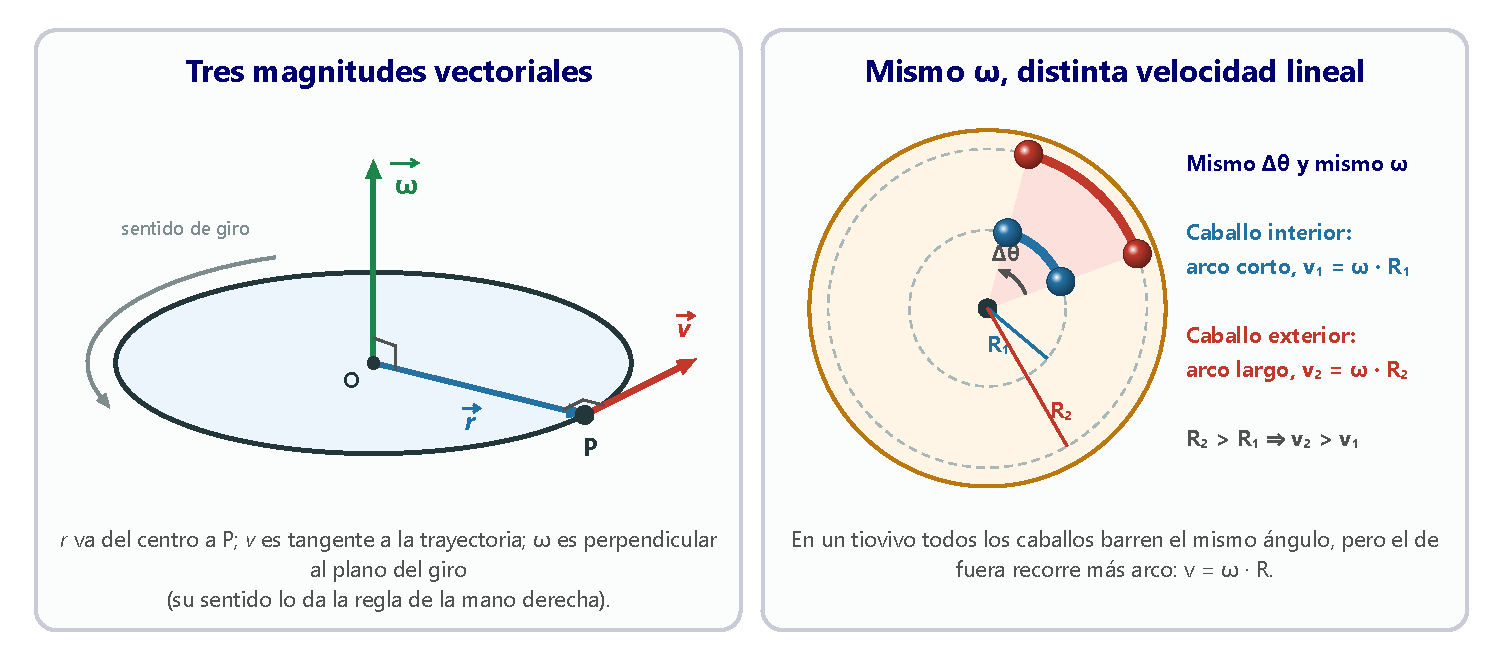
\includegraphics[width=\textwidth]{images/UD9/mcu_vectores}
    \caption{Izquierda: el radio vector, la velocidad lineal y la velocidad angular son vectores. Derecha: en un tiovivo todos los puntos tienen la misma \(\omega\), pero los más alejados del centro tienen más velocidad lineal.}
    \label{fig:mcu_vectores}
\end{figure}

\paragraph{¿Tienen carácter vectorial las magnitudes angulares?} En las fórmulas anteriores usamos solo módulos, pero el radio vector, la velocidad lineal y la velocidad angular son vectores (figura~\ref{fig:mcu_vectores}):
\begin{itemize}
    \item El \textbf{radio vector}, \(\vec{r}\), va del centro de la circunferencia al punto P.
    \item La \textbf{velocidad lineal}, \(\vec{v}\), está aplicada en P, es \textbf{tangente} a la trayectoria y tiene el sentido del movimiento.
    \item La \textbf{velocidad angular}, \(\vec{\omega}\), está aplicada en el centro y es \textbf{perpendicular} al plano de la circunferencia. Su sentido lo da la \textbf{regla de la mano derecha}: si los dedos curvados siguen el giro, el pulgar señala el sentido de \(\vec{\omega}\).
\end{itemize}

\begin{example}
    La Luna da una vuelta alrededor de la Tierra en unos 28 días a una distancia media de \qty{384000}{\km}. Calcula su velocidad angular y su velocidad lineal.
    \[ \omega = \frac{2\pi~\unit{\radian}}{28~\text{días}} \cdot \frac{1~\text{día}}{\qty{86400}{\s}} = \textcolor{red}{\qty{2.6e-6}{\radian\per\s}} \qquad v = \omega \cdot R = \num{2.6e-6} \cdot \qty{3.84e8}{\m} = \textcolor{red}{\qty{997}{\m\per\s}} \]
\end{example}

\begin{example}
    Una plataforma circular de \qty{3}{\m} de radio gira a 15 vueltas por minuto. Calcula la velocidad angular y la velocidad lineal de un punto situado a \qty{1}{\m} del centro y de un punto del borde.
    \[ \omega = \frac{15 \cdot 2\pi~\unit{\radian}}{\qty{60}{\s}} = \frac{\pi}{2}~\unit{\radian\per\s} = \textcolor{red}{\qty{1.57}{\radian\per\s}} \quad \text{(la misma para todos los puntos)} \]
    \[ v_{1\,\mathrm{m}} = \omega \cdot r = \num{1.57} \cdot 1 = \textcolor{red}{\qty{1.6}{\m\per\s}} \qquad v_{3\,\mathrm{m}} = \num{1.57} \cdot 3 = \textcolor{red}{\qty{4.7}{\m\per\s}} \]
\end{example}

\begin{exercise}
    Un satélite artificial da una vuelta a la Tierra cada \qty{5}{\hour} y está a \qty{7570}{\km} del centro de la Tierra. Calcula su velocidad lineal y su velocidad angular.
    \begin{solu}
        \(T = 5 \cdot 3600 = \qty{18000}{\s}\).
        \[ v = \frac{2\pi r}{T} = \frac{2\pi \cdot \qty{7.57e6}{\m}}{\qty{18000}{\s}} = \textcolor{red}{\qty{2642}{\m\per\s}} \qquad \omega = \frac{v}{r} = \frac{2642}{\num{7.57e6}} = \textcolor{red}{\qty{3.5e-4}{\radian\per\s}} \]
    \end{solu}
\end{exercise}

\begin{exercise}
    En una planta embotelladora, una plataforma circular de \qty{25}{\cm} de radio gira a 10 rpm. Calcula la velocidad angular y la velocidad lineal de un punto del borde.
    \begin{solu}
        \[ \omega = \frac{10 \cdot 2\pi~\unit{\radian}}{\qty{60}{\s}} = \frac{\pi}{3}~\unit{\radian\per\s} = \textcolor{red}{\qty{1.05}{\radian\per\s}} \qquad v = \omega \cdot R = \num{1.05} \cdot \qty{0.25}{\m} = \textcolor{red}{\qty{0.26}{\m\per\s}} \]
    \end{solu}
\end{exercise}

\subsection{¿Cuánto tarda en dar una vuelta? Período y frecuencia}

\begin{definition}[Período y frecuencia]
    El \textbf{período}, \(T\), de un MCU es el tiempo que tarda el móvil en dar una vuelta completa. Se mide en segundos.

    La \textbf{frecuencia}, \(f\), es el número de vueltas que da en la unidad de tiempo. Se mide en \textbf{hercios} (\unit{\hertz}): \qty{1}{\hertz} es una vuelta por segundo (\(\unit{\hertz} = \unit{\per\s}\)).

    Son magnitudes inversas:
    \[ T = \frac{1}{f} \qquad\qquad f = \frac{1}{T} \]
\end{definition}

En un período, el móvil recorre la circunferencia completa, \(2\pi R\), y su radio vector barre \(2\pi\) radianes. Por tanto:
\[ v = \frac{2\pi R}{T} = 2\pi R f \qquad\qquad \omega = \frac{2\pi}{T} = 2\pi f \]

\begin{example}
    En un tocadiscos antiguo, un disco de \qty{30}{\cm} de diámetro gira a 33 rpm. Calcula: a) la velocidad angular en \unit{\radian\per\s}; b) la frecuencia y el período; c) la velocidad lineal de un punto del borde.

    a) \(\omega = \dfrac{33 \cdot 2\pi~\unit{\radian}}{\qty{60}{\s}} = \textcolor{red}{\qty{3.46}{\radian\per\s}}\)

    b) \(f = \dfrac{33~\text{vueltas}}{\qty{60}{\s}} = \textcolor{red}{\qty{0.55}{\hertz}}\); \(T = \dfrac{1}{f} = \textcolor{red}{\qty{1.82}{\s}}\)

    c) \(v = \dfrac{2\pi R}{T} = \dfrac{2\pi \cdot \qty{0.15}{\m}}{\qty{1.82}{\s}} = \textcolor{red}{\qty{0.52}{\m\per\s}}\)
\end{example}

\begin{exercise}
    Comprueba que la igualdad \(v = \omega \cdot r\) es homogénea y escribe la ecuación de dimensiones del período y de la frecuencia.
    \begin{solu}
        \([v] = \mathrm{L} \cdot \mathrm{T}^{-1}\); \([\omega] \cdot [r] = \mathrm{T}^{-1} \cdot \mathrm{L}\): los dos miembros tienen las mismas dimensiones, así que \textcolor{red}{es homogénea}. \([T] = \textcolor{red}{\mathrm{T}}\) y \([f] = \textcolor{red}{\mathrm{T}^{-1}}\).
    \end{solu}
\end{exercise}

\begin{exercise}
    Una rueda de \qty{90}{\cm} de diámetro gira a \qty{75}{\radian\per\s}. Calcula el período y la velocidad lineal de un punto de su borde.
    \begin{solu}
        \[ T = \frac{2\pi}{\omega} = \frac{2\pi}{75} = \textcolor{red}{\qty{0.084}{\s}} \qquad v = \omega \cdot R = 75 \cdot \qty{0.45}{\m} = \textcolor{red}{\qty{33.75}{\m\per\s}} \]
    \end{solu}
\end{exercise}

\begin{exercise}
    Una rueda de \qty{1}{\m} de radio gira a 120 vueltas por minuto. Calcula:
    \begin{enumerate}[label=\alph*)]
        \item La frecuencia y el período del movimiento.
        \item La velocidad de un punto del borde de la rueda.
    \end{enumerate}
    \begin{solu}
        a) \(f = \dfrac{120~\text{vueltas}}{\qty{60}{\s}} = \textcolor{red}{\qty{2}{\hertz}}\); \(T = \dfrac{1}{f} = \textcolor{red}{\qty{0.5}{\s}}\).
        b) \(v = \dfrac{2\pi R}{T} = \dfrac{2\pi \cdot 1}{\num{0.5}} = 4\pi = \textcolor{red}{\qty{12.6}{\m\per\s}}\).
    \end{solu}
\end{exercise}

\subsection*{Actividades de consolidación: características del MCU}

\begin{exercise}
    Define qué es el movimiento circular uniforme, el radio vector y el desplazamiento angular.
    \begin{solu}
        El \textcolor{red}{MCU} es el de un cuerpo que describe una circunferencia recorriendo arcos iguales en tiempos iguales. El \textcolor{red}{radio vector} es el vector que va desde el centro de la circunferencia hasta la posición del móvil. El \textcolor{red}{desplazamiento angular} es el ángulo que barre el radio vector entre dos instantes, \(\Delta\theta = \theta_2 - \theta_1\).
    \end{solu}
\end{exercise}

\begin{exercise}
    Una niña montada en un tiovivo barre ángulos de \ang{90}, \ang{180} y \ang{360} a los 5, 10 y 20 segundos de empezar a girar. Calcula:
    \begin{enumerate}[label=\alph*)]
        \item Los radianes que ha barrido en cada caso.
        \item El tiempo que tarda en dar una vuelta.
        \item Su velocidad angular.
    \end{enumerate}
    \begin{solu}
        a) \textcolor{red}{\(\pi/2\) rad}, \textcolor{red}{\(\pi\) rad} y \textcolor{red}{\(2\pi\) rad}. b) \(T = \textcolor{red}{\qty{20}{\s}}\). c) \(\omega = \dfrac{2\pi}{20} = \dfrac{\pi}{10} = \textcolor{red}{\qty{0.31}{\radian\per\s}}\).
    \end{solu}
\end{exercise}

\begin{exercise}
    Un cuerpo con MCU está en el instante \(t_1\) en un punto P\(_1\) cuyo radio vector forma \ang{45} con el eje X, y en el instante \(t_2\), en P\(_2\), a \ang{120}. Calcula el ángulo barrido en grados y en radianes.
    \begin{solu}
        \(\Delta\theta = \ang{120} - \ang{45} = \textcolor{red}{\ang{75}}\). En radianes: \(75 \cdot \dfrac{\pi}{180} = \dfrac{5\pi}{12} = \textcolor{red}{\qty{1.31}{\radian}}\).
    \end{solu}
\end{exercise}

\begin{exercise}
    Una noria gira con MCU a \(\pi/30\) rad/s. Calcula:
    \begin{enumerate}[label=\alph*)]
        \item El ángulo que barre en \qty{6}{\s}.
        \item El tiempo que tardas en dar una vuelta completa montado en una cabina.
    \end{enumerate}
    \begin{solu}
        a) \(\theta = \omega \cdot t = \dfrac{\pi}{30} \cdot 6 = \textcolor{red}{\dfrac{\pi}{5}~\unit{\radian}}\) (\ang{36}). b) \(T = \dfrac{2\pi}{\omega} = \dfrac{2\pi}{\pi/30} = \textcolor{red}{\qty{60}{\s}}\).
    \end{solu}
\end{exercise}

\begin{exercise}
    Un arco de una circunferencia de \qty{20}{\cm} de radio mide \qty{60}{\cm}. Calcula el ángulo correspondiente en radianes y en grados.
    \begin{solu}
        \(\Delta\theta = \dfrac{\Delta s}{R} = \dfrac{60}{20} = \textcolor{red}{\qty{3}{\radian}}\); en grados, \(3 \cdot \dfrac{180}{\pi} = \textcolor{red}{\ang{171.9}}\).
    \end{solu}
\end{exercise}

\begin{exercise}
    Un móvil con MCU da una vuelta completa cada \qty{5}{\s}. Calcula:
    \begin{enumerate}[label=\alph*)]
        \item Su velocidad angular en rad/s, rps y rpm.
        \item El ángulo que barre en \qty{45}{\s}.
    \end{enumerate}
    \begin{solu}
        a) \(\omega = \dfrac{2\pi}{5} = \textcolor{red}{\qty{1.26}{\radian\per\s}} = \textcolor{red}{\num{0.2}~\text{rps}} = \textcolor{red}{12~\text{rpm}}\). b) En \qty{45}{\s} da 9 vueltas: \(\theta = 9 \cdot 2\pi = \textcolor{red}{18\pi~\unit{\radian}}\).
    \end{solu}
\end{exercise}

\begin{exercise}
    Completa la tabla en tu cuaderno:
    \begin{center}
        % --- tabla antigua ---
        % \begin{tblr}{colspec={lccccc}, hlines, vlines, column{1}={bg=ocre!85, fg=white, font=\bfseries}}
            % rpm & 120 & & & & \\
            % rps & & 60 & & 10 & \\
            % rad/s & & & \(\pi\) & & \(\pi/4\) \\
        % \end{tblr}
        % --- tabla nueva ---
        \begin{tabular}{@{}lccccc@{}}
            \toprule
            \textbf{rpm} & 120 &  &  &  &  \\[3pt]
            \textbf{rps} &  & 60 &  & 10 &  \\[3pt]
            \textbf{rad/s} &  &  & \(\pi\) &  & \(\pi/4\) \\
            \bottomrule
        \end{tabular}
    \end{center}
    \begin{solu}
        Se usa que 1 rps = 60 rpm = \(2\pi\) rad/s. Por columnas: 120 rpm = \textcolor{red}{2 rps} = \textcolor{red}{\(4\pi\) rad/s}; 60 rps = \textcolor{red}{3600 rpm} = \textcolor{red}{\(120\pi\) rad/s}; \(\pi\) rad/s = \textcolor{red}{\num{0.5} rps} = \textcolor{red}{30 rpm}; 10 rps = \textcolor{red}{600 rpm} = \textcolor{red}{\(20\pi\) rad/s}; \(\pi/4\) rad/s = \textcolor{red}{1/8 rps} = \textcolor{red}{\num{7.5} rpm}.
    \end{solu}
\end{exercise}

\begin{exercise}
    El extremo del aspa de un ventilador gira con MCU a 60 rpm.
    \begin{enumerate}[label=\alph*)]
        \item Expresa esta velocidad en rad/s.
        \item Calcula el ángulo que barre en \qty{10}{\s}.
        \item Calcula el tiempo que tarda en dar una vuelta.
    \end{enumerate}
    \begin{solu}
        a) \(\omega = \dfrac{60 \cdot 2\pi}{60} = \textcolor{red}{2\pi~\unit{\radian\per\s}}\). b) \(\theta = 2\pi \cdot 10 = \textcolor{red}{20\pi~\unit{\radian}}\). c) \(T = \dfrac{2\pi}{2\pi} = \textcolor{red}{\qty{1}{\s}}\).
    \end{solu}
\end{exercise}

\begin{exercise}
    Un tiovivo gira a 3 rpm. Calcula la velocidad lineal de un niño situado a \qty{75}{\cm}, a \qty{1.5}{\m} y a \qty{2.5}{\m} del centro.
    \begin{solu}
        \(\omega = \dfrac{3 \cdot 2\pi}{60} = \dfrac{\pi}{10}~\unit{\radian\per\s}\), la misma para los tres. Con \(v = \omega \cdot r\):
        \(v_1 = \dfrac{\pi}{10} \cdot \num{0.75} = \textcolor{red}{\qty{0.24}{\m\per\s}}\); \(v_2 = \textcolor{red}{\qty{0.47}{\m\per\s}}\); \(v_3 = \textcolor{red}{\qty{0.79}{\m\per\s}}\).
    \end{solu}
\end{exercise}

\begin{exercise}
    Un satélite de observación de órbita baja (LEO) da una vuelta cada \qty{90}{\minute} a \qty{6570}{\km} del centro de la Tierra. Calcula su velocidad lineal, su velocidad angular y su frecuencia.
    \begin{solu}
        \(T = 90 \cdot 60 = \qty{5400}{\s}\).
        \[ f = \frac{1}{T} = \textcolor{red}{\qty{1.85e-4}{\hertz}} \qquad \omega = \frac{2\pi}{T} = \textcolor{red}{\qty{1.16e-3}{\radian\per\s}} \]
        \[ v = \frac{2\pi r}{T} = \frac{2\pi \cdot \num{6.57e6}}{5400} = \textcolor{red}{\qty{7644}{\m\per\s}} \]
    \end{solu}
\end{exercise}

\begin{exercise}
    Una plataforma circular de \qty{1}{\m} de radio gira a 30 vueltas por minuto. Calcula el período, la velocidad angular y la velocidad lineal de un punto del borde.
    \begin{solu}
        \(f = \dfrac{30}{60} = \qty{0.5}{\hertz} \Rightarrow T = \textcolor{red}{\qty{2}{\s}}\); \(\omega = \dfrac{2\pi}{T} = \textcolor{red}{\qty{3.14}{\radian\per\s}}\); \(v = \omega \cdot R = \textcolor{red}{\qty{3.14}{\m\per\s}}\).
    \end{solu}
\end{exercise}

\begin{exercise}
    La rueda de un coche, de \qty{80}{\cm} de diámetro, gira a 716 rpm. Calcula:
    \begin{enumerate}[label=\alph*)]
        \item La velocidad angular en rad/s.
        \item La velocidad lineal de un punto del borde de la rueda.
        \item El período y la frecuencia.
    \end{enumerate}
    \begin{solu}
        a) \(\omega = \dfrac{716 \cdot 2\pi}{60} = \textcolor{red}{\qty{75}{\radian\per\s}}\). b) \(v = \omega \cdot R = 75 \cdot \num{0.40} = \textcolor{red}{\qty{30}{\m\per\s}}\) (\qty{108}{\km\per\hour}, la velocidad del coche). c) \(f = \dfrac{716}{60} = \textcolor{red}{\qty{11.9}{\hertz}}\); \(T = \dfrac{1}{f} = \textcolor{red}{\qty{0.084}{\s}}\).
    \end{solu}
\end{exercise}

\begin{exercise}
    Una rueda gira a 90 rpm. Calcula la velocidad angular y la velocidad lineal de:
    \begin{enumerate}[label=\alph*)]
        \item Un punto a \qty{10}{\cm} del centro.
        \item Un punto a \qty{20}{\cm} del centro.
        \item El punto central de la rueda.
    \end{enumerate}
    \begin{solu}
        La velocidad angular es la misma en todos los puntos: \(\omega = \dfrac{90 \cdot 2\pi}{60} = 3\pi = \textcolor{red}{\qty{9.42}{\radian\per\s}}\).
        a) \(v = \num{9.42} \cdot \num{0.10} = \textcolor{red}{\qty{0.94}{\m\per\s}}\). b) \(v = \textcolor{red}{\qty{1.88}{\m\per\s}}\). c) \(r = 0 \Rightarrow v = \textcolor{red}{0}\).
    \end{solu}
\end{exercise}

%========================================================================================
\section[La aceleración centrípeta]{¿Puede un movimiento ser uniforme y tener aceleración? La aceleración centrípeta}
%========================================================================================

Sí. El MCU es uniforme porque el módulo de la velocidad no cambia, pero tiene aceleración porque la dirección de la velocidad cambia constantemente.

\subsection{La aceleración centrípeta}

\begin{figure}[H]
    \centering
    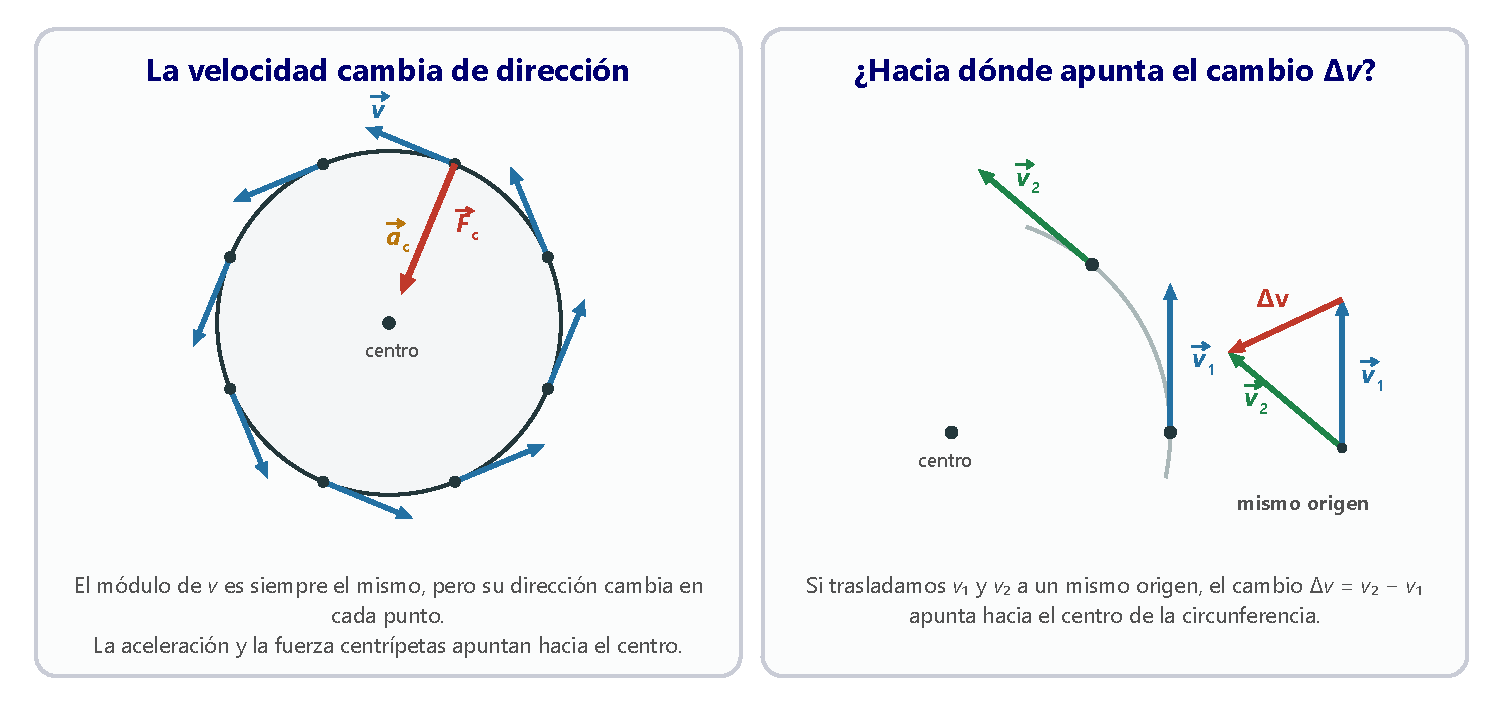
\includegraphics[width=\textwidth]{images/UD9/aceleracion_centripeta}
    \caption{En el MCU la velocidad cambia de dirección en cada punto; ese cambio apunta hacia el centro.}
    \label{fig:aceleracion_centripeta}
\end{figure}

Observa la figura~\ref{fig:aceleracion_centripeta}: el vector velocidad es tangente a la trayectoria en cada punto. Todos los vectores miden lo mismo, pero ninguno apunta en la misma dirección que otro.

\begin{marker}
    En un MCU, el \textbf{módulo} de la velocidad lineal es constante, pero su \textbf{dirección y sentido cambian continuamente}.
\end{marker}

Siempre que cambia la velocidad hay aceleración. Esta se llama \textbf{aceleración centrípeta} o \textbf{normal}, porque es perpendicular a la trayectoria y apunta hacia el \textbf{centro} de la circunferencia. Su módulo es:
\[ a_c = \frac{v^2}{r} \]
donde \(r\) es el radio de la circunferencia. Cuanto más rápido se gira y más cerrada es la curva, mayor es la aceleración centrípeta.

\subsection{¿Qué fuerza produce la aceleración centrípeta? La fuerza centrípeta}

Según la segunda ley de Newton, toda aceleración la produce una fuerza que tiene su misma dirección y sentido. Para que un cuerpo describa un MCU, sobre él tiene que actuar una fuerza dirigida hacia el centro: la \textbf{fuerza centrípeta}, \(\vec{F}_c\).

\begin{definition}[Fuerza centrípeta]
    Es la fuerza resultante, dirigida hacia el centro de la trayectoria, que hace que un cuerpo describa un movimiento circular. Su módulo es:
    \[ F_c = m \cdot a_c = m \cdot \frac{v^2}{r} \]
\end{definition}

La fuerza centrípeta no es una fuerza nueva, sino el papel que cumple alguna fuerza conocida: la tensión de una cuerda, el rozamiento de los neumáticos, la fuerza que hacen las paredes de un tambor o la atracción gravitatoria, como veremos.

\begin{example}
    Un coche de \qty{500}{\kg} toma una curva de \qty{200}{\m} de radio a \qty{72}{\km\per\hour}. Calcula la fuerza centrípeta. ¿Cuáles son su dirección y su sentido?

    Pasamos la velocidad al SI: \(v = 72 \cdot \dfrac{1000}{3600} = \qty{20}{\m\per\s}\).
    \[ F_c = m \cdot \frac{v^2}{r} = \qty{500}{\kg} \cdot \frac{(\qty{20}{\m\per\s})^2}{\qty{200}{\m}} = \textcolor{red}{\qty{1000}{\newton}} \]
    Su dirección es la del radio de la curva y su sentido, \textcolor{red}{hacia el centro} de la curva. En este caso la produce el rozamiento entre los neumáticos y el asfalto.
\end{example}

\begin{exercise}
    Comprueba que las expresiones de la aceleración centrípeta y de la fuerza centrípeta son homogéneas.
    \begin{solu}
        \([a_c] = \dfrac{[v]^2}{[r]} = \dfrac{\mathrm{L}^2\mathrm{T}^{-2}}{\mathrm{L}} = \textcolor{red}{\mathrm{L} \cdot \mathrm{T}^{-2}}\), que son las dimensiones de una aceleración. \([F_c] = \mathrm{M} \cdot \mathrm{L} \cdot \mathrm{T}^{-2}\), las de una fuerza.
    \end{solu}
\end{exercise}

\begin{exercise}
    ¿Existe aceleración centrípeta en un movimiento rectilíneo?
    \begin{solu}
        \textcolor{red}{No}. La aceleración centrípeta aparece cuando cambia la dirección de la velocidad, es decir, cuando la trayectoria es curva.
    \end{solu}
\end{exercise}

\begin{exercise}
    Describe cómo son entre sí las direcciones de la velocidad lineal, la aceleración centrípeta y la fuerza centrípeta en un MCU.
    \begin{solu}
        La velocidad lineal es \textcolor{red}{tangente} a la trayectoria. La aceleración y la fuerza centrípetas tienen la \textcolor{red}{misma dirección}, la del radio, son \textcolor{red}{perpendiculares a la velocidad} y apuntan \textcolor{red}{hacia el centro}.
    \end{solu}
\end{exercise}

\begin{exercise}
    Indica si cada afirmación es verdadera o falsa: «Un MCU es uniforme porque\ldots»
    \begin{enumerate}[label=\alph*)]
        \item \ldots no tiene aceleración.
        \item \ldots el módulo de la velocidad lineal es constante.
        \item \ldots no actúa ninguna fuerza sobre el cuerpo.
        \item \ldots la dirección y el sentido de la velocidad cambian continuamente.
        \item \ldots tiene una aceleración dirigida hacia el centro.
    \end{enumerate}
    \begin{solu}
        a) \textcolor{red}{Falsa}: tiene aceleración centrípeta. b) \textcolor{red}{Verdadera}: por eso es uniforme. c) \textcolor{red}{Falsa}: actúa la fuerza centrípeta. d) \textcolor{red}{Verdadera}, aunque no es la razón de que sea uniforme. e) \textcolor{red}{Verdadera}, aunque tampoco es la razón de que sea uniforme.
    \end{solu}
\end{exercise}

\subsection{¿Qué ocurre cuando deja de actuar la fuerza centrípeta?}

Según la primera ley de Newton, si sobre un cuerpo no actúa ninguna fuerza neta, permanece en reposo o se mueve en línea recta con velocidad constante. Por eso, si la fuerza centrípeta desaparece, el cuerpo \textbf{sale en línea recta, tangente} a la circunferencia, con la velocidad que tenía en ese momento (figura~\ref{fig:sin_fuerza_centripeta}).

\begin{figure}[H]
    \centering
    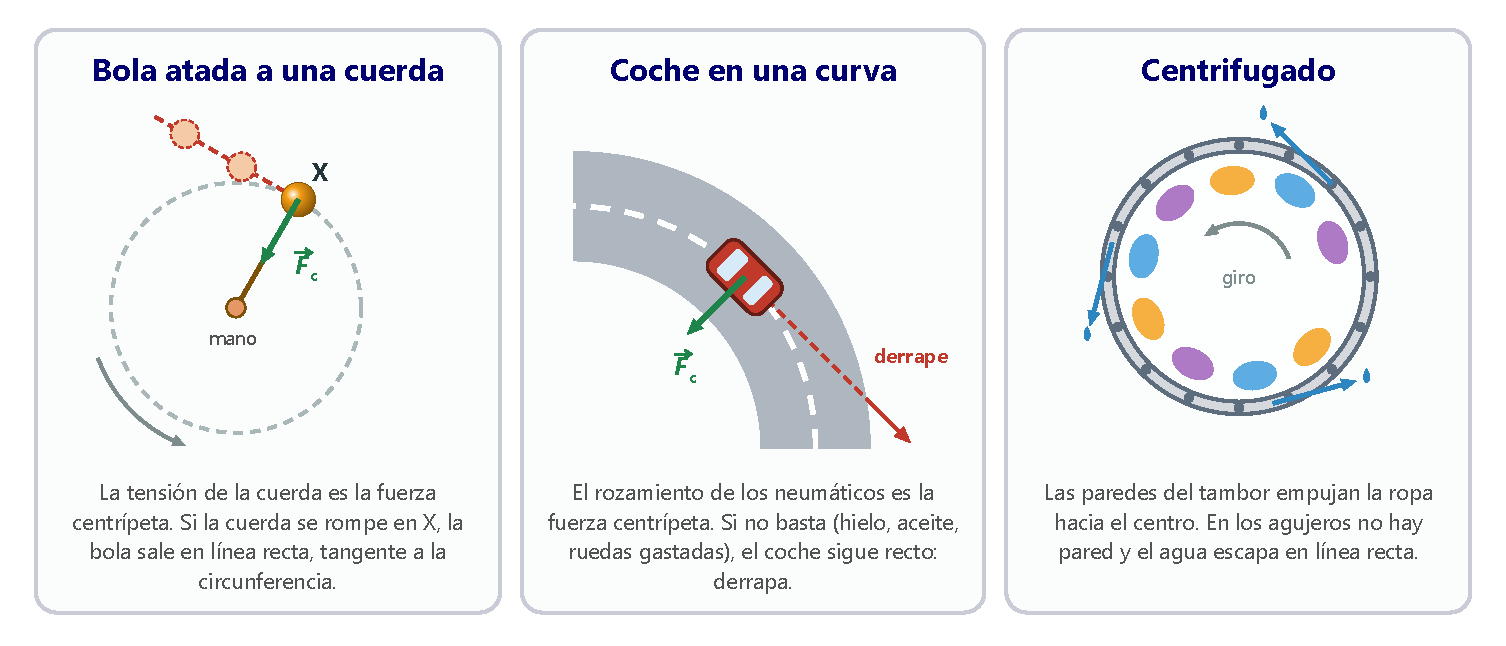
\includegraphics[width=\textwidth]{images/UD9/sin_fuerza_centripeta}
    \caption{Tres situaciones en las que falta la fuerza centrípeta y el cuerpo sigue en línea recta.}
    \label{fig:sin_fuerza_centripeta}
\end{figure}

\begin{exercise}
    Una pelota de \qty{250}{\g} atada a una cuerda de \qty{1}{\m} gira con una velocidad de \qty{1}{\m\per\s}. Calcula el módulo, la dirección y el sentido de la fuerza centrípeta. ¿Qué le pasa a la pelota si se rompe la cuerda?
    \begin{solu}
        \[ F_c = m \cdot \frac{v^2}{r} = \qty{0.25}{\kg} \cdot \frac{(\qty{1}{\m\per\s})^2}{\qty{1}{\m}} = \textcolor{red}{\qty{0.25}{\newton}} \]
        Tiene la dirección de la cuerda y sentido hacia la mano (el centro). Si la cuerda se rompe, la pelota \textcolor{red}{sale en línea recta, tangente} a la circunferencia.
    \end{solu}
\end{exercise}

\begin{exercise}
    Un coche de \qty{650}{\kg} toma una curva de \qty{200}{\m} de radio a \qty{90}{\km\per\hour}. Calcula el módulo de la fuerza centrípeta.
    \begin{solu}
        \(v = \qty{90}{\km\per\hour} = \qty{25}{\m\per\s}\).
        \[ F_c = m \cdot \frac{v^2}{r} = 650 \cdot \frac{25^2}{200} = \textcolor{red}{\qty{2031}{\newton}} \]
    \end{solu}
\end{exercise}

\subsection*{Actividades de consolidación: la aceleración y la fuerza centrípetas}

\begin{exercise}
    En la «esfera de la muerte» del circo, los motoristas dan vueltas por dentro de una gran esfera de rejilla. ¿Qué fuerza les permite girar sin caerse?
    \begin{solu}
        La \textcolor{red}{fuerza centrípeta}, que en este caso la ejerce la pared de la esfera sobre la moto (con la ayuda del peso en la parte alta).
    \end{solu}
\end{exercise}

\begin{exercise}
    Un motorista gira dentro de una esfera de \qty{3}{\m} de radio describiendo un círculo vertical. ¿Cuál es la velocidad mínima que debe llevar en el punto más alto para no caer? Ten en cuenta que caerá si su peso es mayor que la fuerza centrípeta necesaria (\(g = \qty{9.8}{\m\per\square\s}\)).
    \begin{solu}
        En el límite, el peso es justo la fuerza centrípeta:
        \[ m \cdot g = m \cdot \frac{v^2}{r} \quad\Rightarrow\quad v = \sqrt{g \cdot r} = \sqrt{\num{9.8} \cdot 3} = \textcolor{red}{\qty{5.4}{\m\per\s}} \]
    \end{solu}
\end{exercise}

\begin{exercise}
    Investiga en qué deportes y atracciones de feria tiene un papel protagonista la fuerza centrípeta.
    \begin{solu}
        Respuesta libre. Por ejemplo, el \textcolor{red}{lanzamiento de martillo}, el ciclismo en pista (velódromo con curvas peraltadas), el patinaje, las curvas en el automovilismo, las sillas voladoras, la noria o las montañas rusas con bucles.
    \end{solu}
\end{exercise}

\begin{exercise}
    Completa la frase con las palabras \emph{dirección} y \emph{módulo}: «La fuerza centrípeta provoca un cambio en la \ldots{} de la velocidad, pero no en su \ldots».
    \begin{solu}
        «La fuerza centrípeta provoca un cambio en la \textcolor{red}{dirección} de la velocidad, pero no en su \textcolor{red}{módulo}».
    \end{solu}
\end{exercise}

\begin{exercise}
    ¿Verdadero o falso? Justifícalo: «La fuerza que actúa sobre un cuerpo tiene siempre la dirección de su movimiento».
    \begin{solu}
        \textcolor{red}{Falso}. En el movimiento circular, la fuerza centrípeta es perpendicular a la velocidad.
    \end{solu}
\end{exercise}

\begin{exercise}
    Una bola atada a una cuerda gira en un plano horizontal.
    \begin{enumerate}[label=\alph*)]
        \item Completa: «La fuerza que obliga a la bola a describir una circunferencia se llama fuerza \ldots{} Si esta fuerza desaparece, la bola se mueve en línea \ldots, como predice la primera ley de Newton».
        \item ¿Hay que hacer más o menos fuerza si la masa de la bola es mayor? ¿Y si la velocidad es mayor? ¿Y si el radio es menor?
        \item Dibuja la trayectoria de la bola si la cuerda se rompe en un punto X.
    \end{enumerate}
    \begin{solu}
        a) Fuerza \textcolor{red}{centrípeta}; en línea \textcolor{red}{recta}. b) Hay que hacer \textcolor{red}{más fuerza} en los tres casos, porque \(F_c = m v^2 / r\). c) La bola sale en línea recta, \textcolor{red}{tangente} a la circunferencia en X (figura~\ref{fig:sin_fuerza_centripeta}).
    \end{solu}
\end{exercise}

\begin{exercise}
    Calcula la fuerza centrípeta de la actividad anterior si la bola tiene \qty{1}{\kg}, el radio es \qty{1}{\m} y la velocidad, \qty{1}{\m\per\s}.
    \begin{solu}
        \(F_c = m \cdot \dfrac{v^2}{r} = 1 \cdot \dfrac{1^2}{1} = \textcolor{red}{\qty{1}{\newton}}\).
    \end{solu}
\end{exercise}

\begin{exercise}
    Una esfera de \qty{1.5}{\kg} describe una circunferencia de \qty{0.5}{\m} de radio a \qty{2}{\m\per\s}. Calcula la fuerza centrípeta.
    \begin{solu}
        \(F_c = \num{1.5} \cdot \dfrac{2^2}{\num{0.5}} = \textcolor{red}{\qty{12}{\newton}}\).
    \end{solu}
\end{exercise}

\begin{exercise}
    Describe qué le sucede a un cuerpo que se mueve en línea recta si actúa sobre él una fuerza constante:
    \begin{enumerate}[label=\alph*)]
        \item Con la misma dirección y sentido que el movimiento.
        \item Siempre perpendicular al movimiento.
    \end{enumerate}
    \begin{solu}
        a) Sigue en línea recta, pero cada vez más deprisa: \textcolor{red}{MRUA}. b) Cambia de dirección sin cambiar de rapidez: \textcolor{red}{MCU}.
    \end{solu}
\end{exercise}

\begin{exercise}
    Calcula la fuerza centrípeta que actúa sobre una bola de \qty{350}{\g} atada a una cuerda de \qty{1}{\m} que gira a \qty{4}{\m\per\s}.
    \begin{solu}
        \(F_c = \num{0.350} \cdot \dfrac{4^2}{1} = \textcolor{red}{\qty{5.6}{\newton}}\).
    \end{solu}
\end{exercise}

\begin{exercise}
    Un cuerpo de \qty{1.5}{\kg} recorre una circunferencia de \qty{50}{\cm} de radio a 2 rps. Calcula la fuerza centrípeta e indica su dirección y sentido.
    \begin{solu}
        \(\omega = 2 \cdot 2\pi = 4\pi~\unit{\radian\per\s}\); \(v = \omega \cdot r = 4\pi \cdot \num{0.5} = 2\pi~\unit{\m\per\s}\).
        \[ F_c = m \cdot \frac{v^2}{r} = \num{1.5} \cdot \frac{(2\pi)^2}{\num{0.5}} = \textcolor{red}{\qty{118}{\newton}} \]
        Dirección: la del radio; sentido: \textcolor{red}{hacia el centro} de la circunferencia.
    \end{solu}
\end{exercise}

%========================================================================================
\section{El universo mecánico: las leyes de Kepler}
%========================================================================================

En el siglo \textsc{xvi}, \textbf{Nicolás Copérnico} propuso el \textbf{modelo heliocéntrico}: la Tierra no está quieta en el centro del universo, sino que gira, como los demás planetas, alrededor del Sol; el único astro que gira alrededor de la Tierra es la Luna. A comienzos del siglo \textsc{xvii}, \textbf{Johannes Kepler}, a partir de las precisas observaciones de \textbf{Tycho Brahe}, enunció tres leyes que describen cómo se mueven los planetas.

\begin{figure}[H]
    \centering
    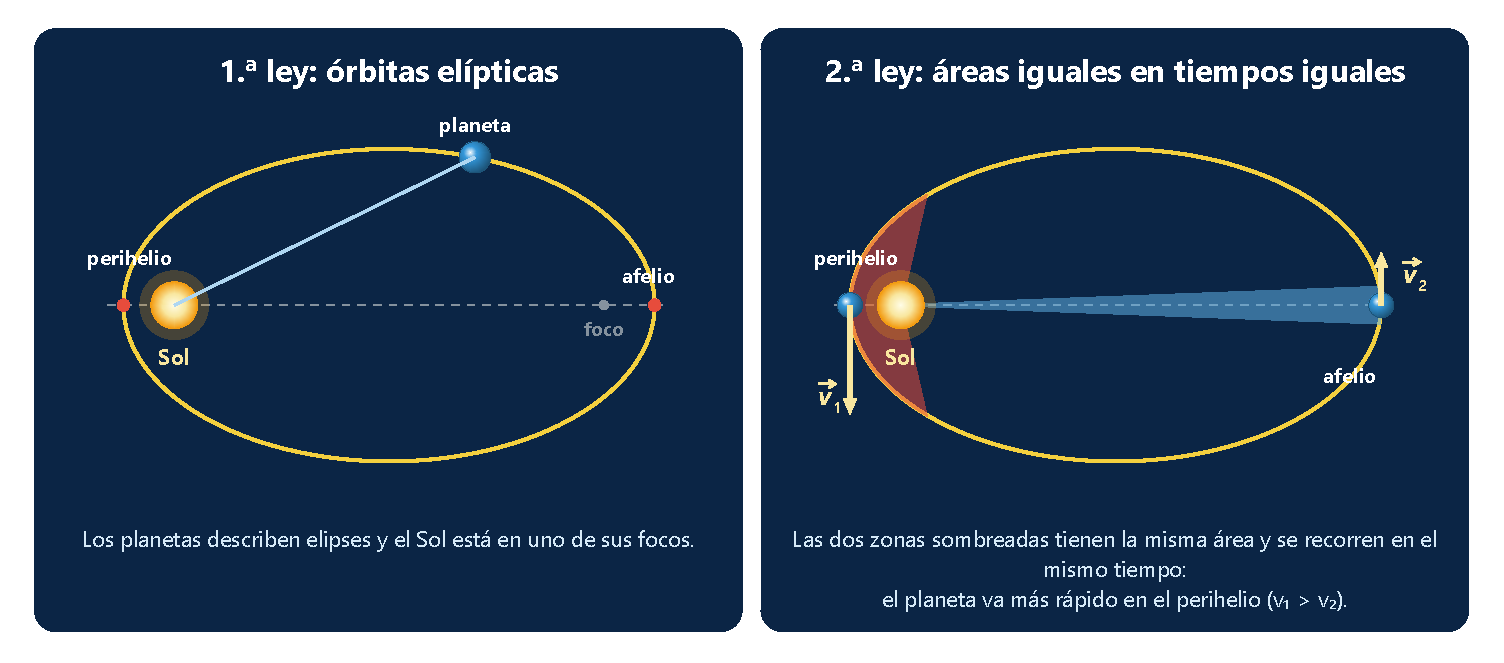
\includegraphics[width=\textwidth]{images/UD9/leyes_kepler}
    \caption{Primera y segunda leyes de Kepler (la elipse está muy exagerada: las órbitas reales son casi circulares).}
    \label{fig:leyes_kepler}
\end{figure}

\begin{definition}[Leyes de Kepler]
    \textbf{Primera ley.} Los planetas giran alrededor del Sol describiendo \textbf{órbitas elípticas}, y el Sol está en uno de los focos de la elipse. El punto de la órbita más cercano al Sol se llama \textbf{perihelio}, y el más alejado, \textbf{afelio}.

    \textbf{Segunda ley.} El radio vector que une el Sol con el planeta barre \textbf{áreas iguales en tiempos iguales}.

    \textbf{Tercera ley.} Para todos los planetas, el cociente entre el cubo del radio medio de la órbita y el cuadrado del período es constante:
    \[ \frac{r^3_{\text{Mercurio}}}{T^2_{\text{Mercurio}}} = \frac{r^3_{\text{Venus}}}{T^2_{\text{Venus}}} = \frac{r^3_{\text{Tierra}}}{T^2_{\text{Tierra}}} = \ldots = \text{constante} \]
\end{definition}

La segunda ley implica que la rapidez del planeta \textbf{no es constante}: es mayor en el perihelio que en el afelio (figura~\ref{fig:leyes_kepler}). La tercera ley dice que cuanto más lejos está un planeta del Sol, más tarda en dar una vuelta.

\begin{remark}
    \textbf{Unidades para medir distancias en el universo.} La \textbf{unidad astronómica} (UA) es la distancia media entre la Tierra y el Sol: \(1~\text{UA} \approx \qty{1.5e11}{\m}\). El \textbf{año luz} es la distancia que recorre la luz en un año: \(\num{9.46e12}~\unit{\km}\).
\end{remark}

\begin{example}
    El cometa Halley tarda unos 76 años en dar una vuelta alrededor del Sol. Calcula su distancia media al Sol, sabiendo que la de la Tierra es \qty{1.5e11}{\m} y su período, 1 año.

    Aplicamos la tercera ley de Kepler a la Tierra y al cometa (podemos dejar los períodos en años):
    \[ \frac{(\qty{1.5e11}{\m})^3}{(1~\text{año})^2} = \frac{r^3_{\text{H}}}{(76~\text{años})^2} \quad\Rightarrow\quad r_{\text{H}} = \sqrt[3]{76^2 \cdot (\num{1.5e11})^3} = \textcolor{red}{\qty{2.69e12}{\m}} \]
\end{example}

\begin{exercise}
    ¿Qué explican las leyes de Kepler: cómo se mueven los planetas o por qué lo hacen?
    \begin{solu}
        Explican \textcolor{red}{cómo se mueven}, no por qué. La causa del movimiento la explicó Newton con la ley de gravitación universal.
    \end{solu}
\end{exercise}

\begin{exercise}
    El radio de la órbita de la Tierra es \qty{1.49e11}{\m} y el de Urano, \qty{2.87e12}{\m}. Expresa estas distancias en UA y calcula el período de Urano en años terrestres.
    \begin{solu}
        La Tierra está a \textcolor{red}{1 UA} y Urano a \(\num{2.87e12}/\num{1.49e11} = \textcolor{red}{\num{19.26}~\text{UA}}\). Con la tercera ley, midiendo en UA y años, la constante vale 1 (la de la Tierra):
        \[ \frac{\num{19.26}^3}{T^2} = \frac{1^3}{1^2} \quad\Rightarrow\quad T = \sqrt{\num{19.26}^3} = \textcolor{red}{\num{84.5}~\text{años}} \]
    \end{solu}
\end{exercise}

\subsection*{Actividades de consolidación: las leyes de Kepler}

\begin{exercise}
    En tiempos de Copérnico ya se conocían las distancias de los planetas al Sol tomando como unidad la distancia Tierra-Sol:
    \begin{center}
        % --- tabla antigua ---
        % \begin{tblr}{colspec={lcccccc}, hlines, vlines, row{1}={bg=ocre!85, fg=white, font=\bfseries}, cell{1}{1}={bg=ocre!85, fg=white}}
            % Planeta & Mercurio & Venus & Tierra & Marte & Júpiter & Saturno \\
            % Distancia al Sol & \num{0.389} & \num{0.724} & 1 & \num{1.525} & \num{5.200} & \num{9.510} \\
        % \end{tblr}
        % --- tabla nueva ---
        \begin{tabular}{@{}lcccccc@{}}
            \toprule
            \textbf{Planeta} & \textbf{Mercurio} & \textbf{Venus} & \textbf{Tierra} & \textbf{Marte} & \textbf{Júpiter} & \textbf{Saturno} \\
            \midrule
            Distancia al Sol & \num{0.389} & \num{0.724} & 1 & \num{1.525} & \num{5.200} & \num{9.510} \\
            \bottomrule
        \end{tabular}
    \end{center}
    Si la distancia Tierra-Sol es \qty{1.5e8}{\km}, calcula la distancia mínima posible entre la Tierra y cada uno de los otros planetas, suponiendo órbitas circulares.
    \begin{solu}
        La distancia mínima se da cuando el planeta y la Tierra están alineados al mismo lado del Sol: es la diferencia de sus distancias al Sol, \(|r - 1| \cdot \num{1.5e8}~\unit{\km}\).
        Mercurio: \(\num{0.611} \cdot \num{1.5e8} = \textcolor{red}{\qty{9.17e7}{\km}}\); Venus: \textcolor{red}{\qty{4.14e7}{\km}}; Marte: \textcolor{red}{\qty{7.88e7}{\km}}; Júpiter: \textcolor{red}{\qty{6.30e8}{\km}}; Saturno: \textcolor{red}{\qty{1.28e9}{\km}}.
    \end{solu}
\end{exercise}

\begin{exercise}
    ¿Verdadero o falso? «El planeta más cercano al Sol es el que tiene el período más corto».
    \begin{solu}
        \textcolor{red}{Verdadero}, según la tercera ley de Kepler: cuanto menor es \(r\), menor es \(T\).
    \end{solu}
\end{exercise}

\begin{exercise}
    Explica con un dibujo la idea de Kepler de que los planetas van más deprisa cuanto más cerca están del Sol. ¿Qué ley la recoge?
    \begin{solu}
        La \textcolor{red}{segunda ley}: el radio vector barre áreas iguales en tiempos iguales. Cerca del Sol (perihelio) el radio vector es corto, así que para barrer la misma área el planeta tiene que recorrer un arco más largo: va \textcolor{red}{más rápido} que en el afelio (figura~\ref{fig:leyes_kepler}).
    \end{solu}
\end{exercise}

\begin{exercise}
    Estos son los radios de las órbitas (en UA) y los períodos que manejaba Kepler. Comprueba con ellos la tercera ley.
    \begin{center}
        % --- tabla antigua ---
        % \begin{tblr}{colspec={lcc}, hlines, vlines, row{1}={bg=ocre!85, fg=white, font=\bfseries}}
            % Planeta & Radio de la órbita (UA) & Período (días) \\
            % Mercurio & \num{0.389} & \num{87.77} \\
            % Venus & \num{0.724} & \num{224.70} \\
            % Tierra & \num{1.000} & \num{365.25} \\
            % Marte & \num{1.525} & \num{686.98} \\
            % Júpiter & \num{5.200} & \num{4332.62} \\
            % Saturno & \num{9.510} & \num{10759.20} \\
        % \end{tblr}
        % --- tabla nueva ---
        \begin{tabular}{@{}lcc@{}}
            \toprule
            \textbf{Planeta} & \textbf{Radio de la órbita (UA)} & \textbf{Período (días)} \\
            \midrule
            Mercurio & \num{0.389} & \num{87.77} \\[3pt]
            Venus & \num{0.724} & \num{224.70} \\[3pt]
            Tierra & \num{1.000} & \num{365.25} \\[3pt]
            Marte & \num{1.525} & \num{686.98} \\[3pt]
            Júpiter & \num{5.200} & \num{4332.62} \\[3pt]
            Saturno & \num{9.510} & \num{10759.20} \\
            \bottomrule
        \end{tabular}
    \end{center}
    \begin{solu}
        Calculamos \(r^3/T^2\) para cada planeta: Mercurio \num{7.64e-6}; Venus \num{7.52e-6}; Tierra \num{7.50e-6}; Marte \num{7.52e-6}; Júpiter \num{7.49e-6}; Saturno \num{7.43e-6} (en UA\(^3\)/día\(^2\)). Son prácticamente iguales, como dice la tercera ley; su valor medio es \textcolor{red}{\(\num{7.5e-6}~\text{UA}^3/\text{día}^2\)}.
    \end{solu}
\end{exercise}

\begin{exercise}
    Imagina que se descubre un planeta diez veces más lejos del Sol que la Tierra. ¿Cuántos años tardaría en dar una vuelta? Usa los datos de la actividad anterior.
    \begin{solu}
        \[ \frac{10^3}{T^2} = \num{7.5e-6} \quad\Rightarrow\quad T = \sqrt{\frac{1000}{\num{7.5e-6}}} = \num{11547}~\text{días} = \textcolor{red}{\num{31.6}~\text{años}} \]
        (También se obtiene directamente: \(T = \sqrt{10^3} = \num{31.6}\) años.)
    \end{solu}
\end{exercise}

\begin{exercise}
    El cometa Swift-Tuttle tiene un período de unos 113 años. Calcula su distancia media al Sol, sabiendo que la de la Tierra es \qty{1.49e11}{\m}.
    \begin{solu}
        \[ \frac{(\num{1.49e11})^3}{1^2} = \frac{r^3}{113^2} \quad\Rightarrow\quad r = \num{1.49e11} \cdot \sqrt[3]{113^2} = \textcolor{red}{\qty{3.48e12}{\m}} \]
    \end{solu}
\end{exercise}

%========================================================================================
\section{La ley de gravitación universal}
%========================================================================================

¿Qué fuerza ejerce el Sol sobre los planetas para que se muevan como dicen las leyes de Kepler? Newton empezó por la Luna. Si sobre ella no actuara ninguna fuerza, se movería en línea recta. Pero describe una órbita casi circular alrededor de la Tierra, así que tiene que haber una fuerza que la atraiga hacia la Tierra. Cuenta la leyenda que, viendo caer una manzana en su jardín, Newton pensó que la fuerza que hace caer la manzana y la que mantiene a la Luna en su órbita son \textbf{la misma}: la Tierra atrae a la Luna igual que atrae a la manzana.

A partir de datos astronómicos y de muchos cálculos, Newton enunció en 1687 la \textbf{ley de gravitación universal}:

\begin{definition}[Ley de gravitación universal]
    Todos los cuerpos del universo se atraen con una fuerza directamente proporcional al producto de sus masas e inversamente proporcional al cuadrado de la distancia que los separa:
    \[ F = G \cdot \frac{m \cdot m'}{r^2} \]
    \(F\) es la fuerza de atracción (\unit{\newton}); \(m\) y \(m'\), las masas de los cuerpos (\unit{\kg}); \(r\), la distancia entre sus centros (\unit{\m}), y \(G\), la \textbf{constante de gravitación universal}:
    \[ G = \qty{6.67e-11}{\newton\square\m\per\square\kg} \]
\end{definition}

\begin{figure}[H]
    \centering
    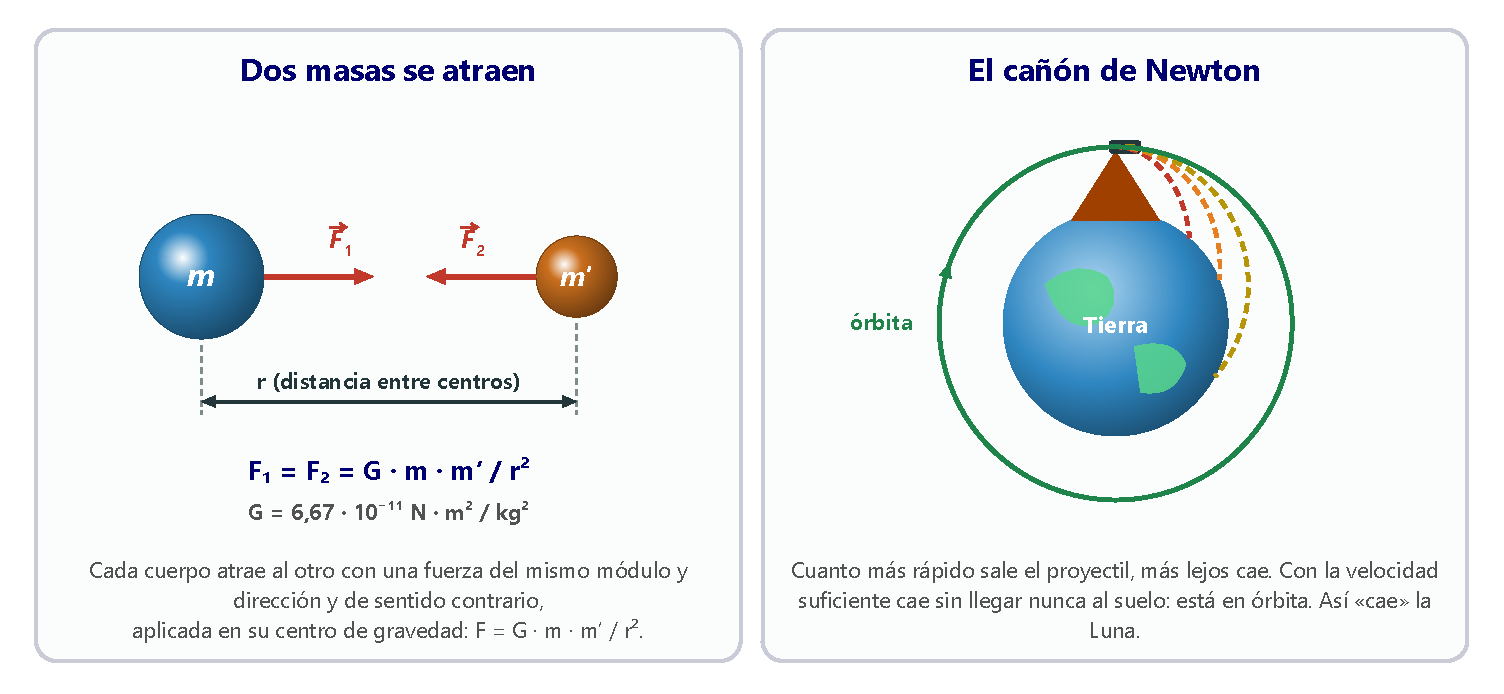
\includegraphics[width=\textwidth]{images/UD9/gravitacion}
    \caption{Izquierda: dos masas se atraen con fuerzas iguales y opuestas. Derecha: el «cañón de Newton»; un proyectil lanzado con la velocidad suficiente queda en órbita.}
    \label{fig:gravitacion}
\end{figure}

\subsection{Características de la fuerza gravitatoria}

\begin{itemize}
    \item Es \textbf{universal}: actúa entre todos los cuerpos que tienen masa.
    \item Es siempre de \textbf{atracción}.
    \item Está aplicada en el \textbf{centro de gravedad} de cada cuerpo y su dirección es la de la \textbf{recta que une sus centros}.
    \item Cumple la tercera ley de Newton: la Tierra atrae al Sol con la misma fuerza con la que el Sol atrae a la Tierra, pero en sentido contrario (figura~\ref{fig:gravitacion}).
    \item Actúa \textbf{a distancia}, sin que los cuerpos estén en contacto, y puede hacer de \textbf{fuerza centrípeta}.
\end{itemize}

\paragraph{¿Es fuerte la fuerza gravitatoria?} \(G\) es muy pequeña, así que la atracción entre dos objetos corrientes es imperceptible: solo se aprecia cuando al menos una de las masas es enorme, como la de un planeta. Las gráficas muestran cómo depende la fuerza de cada variable:
\begin{itemize}
    \item Si la distancia no cambia, la fuerza es \textbf{directamente proporcional} a cada masa: si una masa se duplica, la fuerza se duplica.
    \item Si las masas no cambian, la fuerza es \textbf{inversamente proporcional al cuadrado de la distancia}: si la distancia se duplica, la fuerza se divide entre cuatro. Disminuye muy deprisa al alejarse.
\end{itemize}

\begin{center}
    \begin{tikzpicture}
        \begin{axis}[grafica, width=6.5cm, height=4.6cm, xlabel={masa, \(m\)}, ylabel={fuerza, \(F\)}, xmin=0, xmax=5.2, ymin=0, ymax=5.5, xticklabels={}, yticklabels={}, title={\small \(F\) frente a \(m\) (\(r\) constante)}]
            \addplot[mark=none, domain=0:5, line width=1.4pt, color=red!75!black] {x};
        \end{axis}
    \end{tikzpicture}
    \hspace{0.6cm}
    \begin{tikzpicture}
        \begin{axis}[grafica, width=6.5cm, height=4.6cm, xlabel={distancia, \(r\)}, ylabel={fuerza, \(F\)}, xmin=0, xmax=5.2, ymin=0, ymax=5.5, xticklabels={}, yticklabels={}, title={\small \(F\) frente a \(r\) (masas constantes)}]
            \addplot[mark=none, domain=0.43:5, samples=80, line width=1.4pt, color=red!75!black] {1/x^2};
        \end{axis}
    \end{tikzpicture}
\end{center}

\begin{example}
    Calcula la fuerza de atracción gravitatoria entre el protón y el electrón de un átomo de hidrógeno (\(m_p = \qty{1.67e-27}{\kg}\), \(m_e = \qty{9.1e-31}{\kg}\), distancia \qty{5.3e-11}{\m}).
    \[ F = \num{6.67e-11} \cdot \frac{\num{1.67e-27} \cdot \num{9.1e-31}}{(\num{5.3e-11})^2} = \textcolor{red}{\qty{3.6e-47}{\newton}} \]
\end{example}

\begin{example}
    Calcula la fuerza de atracción entre la Tierra (\qty{5.97e24}{\kg}) y el Sol (\qty{2.0e30}{\kg}), separados \qty{1.5e11}{\m}.
    \[ F = \num{6.67e-11} \cdot \frac{\num{5.97e24} \cdot \num{2.0e30}}{(\num{1.5e11})^2} = \textcolor{red}{\qty{3.5e22}{\newton}} \]
\end{example}

\begin{example}
    ¿Con qué fuerza te atrae la Tierra cuando estás en su superficie (\(R_T = \qty{6.37e6}{\m}\))? Llama \(m\) a tu masa.
    \[ F = \num{6.67e-11} \cdot \frac{\num{5.97e24} \cdot m}{(\num{6.37e6})^2} = \textcolor{red}{\num{9.8} \cdot m}~\unit{\newton} \]
\end{example}

\begin{exercise}
    Compara la intensidad de la atracción gravitatoria entre partículas atómicas y entre cuerpos celestes, usando los dos primeros ejemplos.
    \begin{solu}
        \(\dfrac{\num{3.5e22}}{\num{3.6e-47}} \approx \num{1e69}\): la atracción entre la Tierra y el Sol es unas \textcolor{red}{\(10^{69}\) veces mayor}. Entre partículas, la fuerza gravitatoria es despreciable porque sus masas son minúsculas.
    \end{solu}
\end{exercise}

\begin{exercise}
    Sustituye tu masa en el tercer ejemplo. ¿Qué significado tiene el número \num{9.8} que aparece en el resultado?
    \begin{solu}
        Respuesta libre (por ejemplo, con \qty{60}{\kg}, \(F = \qty{588}{\newton}\)). Esa fuerza es tu \textcolor{red}{peso}, y \num{9.8} es la \textcolor{red}{aceleración de la gravedad}, \(g\), en \unit{\m\per\square\s}.
    \end{solu}
\end{exercise}

\begin{exercise}
    Corrige los enunciados que sean falsos:
    \begin{enumerate}[label=\alph*)]
        \item La constante de gravitación universal depende de dónde estén los cuerpos en el universo.
        \item La Tierra atrae a la Luna con mucha más fuerza que la Luna a la Tierra.
        \item La fuerza gravitatoria puede actuar como fuerza centrípeta sin que los cuerpos estén en contacto.
    \end{enumerate}
    \begin{solu}
        a) Falso: \(G\) \textcolor{red}{es la misma en todo el universo}. b) Falso: las dos fuerzas tienen \textcolor{red}{el mismo módulo} (tercera ley de Newton); lo que ocurre es que a la Luna, con menos masa, esa fuerza le produce más aceleración. c) \textcolor{red}{Verdadero}.
    \end{solu}
\end{exercise}

\begin{exercise}
    En 1797, unos cien años después de que Newton publicara su ley, Henry Cavendish midió el valor de \(G\) con una balanza de torsión. Busca información sobre cómo funciona esa balanza y cómo hizo Cavendish la medida.
    \begin{solu}
        Respuesta libre. Una varilla con dos esferas pequeñas cuelga de un hilo fino; al acercar dos esferas grandes, la atracción gravitatoria hace girar la varilla y retuerce el hilo. Midiendo el ángulo de giro, Cavendish calculó la fuerza y, con ella, \(G\). A esta experiencia se la llamó «pesar la Tierra», porque, conocido \(G\), se puede calcular la masa de la Tierra.
    \end{solu}
\end{exercise}

\begin{exercise}
    El modelo heliocéntrico y la ley de gravitación universal tuvieron varios protagonistas. Investiga las aportaciones de Copérnico, Galileo, Kepler y Newton y el contexto histórico en el que trabajaron.
    \begin{solu}
        Respuesta libre. Copérnico propuso el modelo heliocéntrico (1543); Galileo lo defendió con sus observaciones con el telescopio (satélites de Júpiter, fases de Venus) y fue juzgado por la Inquisición; Kepler descubrió las leyes del movimiento planetario; Newton las explicó con la ley de gravitación universal (1687).
    \end{solu}
\end{exercise}

\subsection*{Actividades de consolidación: la ley de gravitación universal}

\begin{exercise}
    Justifica por qué la atracción gravitatoria disminuye rápidamente al aumentar la distancia entre dos cuerpos.
    \begin{solu}
        Porque es \textcolor{red}{inversamente proporcional al cuadrado de la distancia}: al duplicar la distancia, la fuerza se hace cuatro veces menor; al triplicarla, nueve veces menor.
    \end{solu}
\end{exercise}

\begin{exercise}
    Calcula la fuerza de atracción entre dos cuerpos de \qty{50}{\kg} y \qty{60}{\kg} separados \qty{50}{\cm}.
    \begin{solu}
        \[ F = \num{6.67e-11} \cdot \frac{50 \cdot 60}{\num{0.5}^2} = \textcolor{red}{\qty{8.0e-7}{\newton}} \]
    \end{solu}
\end{exercise}

\begin{exercise}
    Calcula la fuerza con la que se atraen la Tierra y la Luna. Datos: \(M_T = \qty{5.97e24}{\kg}\); \(m_L = \qty{7.20e22}{\kg}\); \(d = \qty{3.84e8}{\m}\).
    \begin{solu}
        \[ F = \num{6.67e-11} \cdot \frac{\num{5.97e24} \cdot \num{7.20e22}}{(\num{3.84e8})^2} = \textcolor{red}{\qty{1.94e20}{\newton}} \]
    \end{solu}
\end{exercise}

\begin{exercise}
    Compara los resultados de las dos actividades anteriores. ¿Qué conclusión sacas?
    \begin{solu}
        La fuerza entre la Tierra y la Luna es unas \(10^{26}\) veces mayor. La gravedad solo es apreciable cuando intervienen \textcolor{red}{masas muy grandes}, como las de los astros.
    \end{solu}
\end{exercise}

\begin{exercise}
    Una masa de \qty{200}{\kg} está a \qty{10}{\m} de otra de \qty{150}{\kg}. ¿Con qué fuerza se atraen? ¿Dónde está aplicada cada fuerza? ¿Cuáles son su dirección y su sentido?
    \begin{solu}
        \[ F = \num{6.67e-11} \cdot \frac{200 \cdot 150}{10^2} = \textcolor{red}{\qty{2.0e-8}{\newton}} \]
        Hay dos fuerzas iguales, una \textcolor{red}{aplicada en el centro de gravedad de cada cuerpo}. Su dirección es la de la recta que une los centros y su sentido, \textcolor{red}{hacia el otro cuerpo}.
    \end{solu}
\end{exercise}

\begin{exercise}
    La Luna (\qty{7.3e22}{\kg}) está a \qty{3.9e8}{\m} del centro de la Tierra (\qty{5.97e24}{\kg}). ¿A qué distancia del centro de la Tierra se anulan las atracciones de los dos astros sobre un cuerpo?
    \begin{solu}
        Llamamos \(x\) a la distancia desde la Tierra; desde la Luna será \(d - x\). Igualamos las dos atracciones (la masa del cuerpo y \(G\) se simplifican):
        \[ \frac{M_T}{x^2} = \frac{m_L}{(d - x)^2} \quad\Rightarrow\quad \frac{x}{d - x} = \sqrt{\frac{M_T}{m_L}} = \sqrt{\frac{\num{5.97e24}}{\num{7.3e22}}} = \num{9.04} \]
        \[ x = \num{9.04} \cdot (d - x) \quad\Rightarrow\quad x = \frac{\num{9.04} \cdot \num{3.9e8}}{\num{10.04}} = \textcolor{red}{\qty{3.51e8}{\m}} \]
        Es decir, a unos \qty{351000}{\km} de la Tierra, mucho más cerca de la Luna, que tiene menos masa.
    \end{solu}
\end{exercise}

%========================================================================================
\section{La síntesis newtoniana}
%========================================================================================

Con sus tres leyes de la dinámica y la ley de gravitación universal, Newton explicó con las mismas ideas fenómenos que hasta entonces parecían no tener nada que ver: la caída de los cuerpos en la Tierra, el movimiento de la Luna, el de los planetas y el de los cometas. A esta unificación se la llama \textbf{síntesis newtoniana}.

\subsection{La caída y el peso de los cuerpos}

Los objetos caen porque la Tierra los atrae: el \textbf{peso} es la fuerza gravitatoria con la que la Tierra atrae a un cuerpo. En la unidad anterior vimos que \(P = m \cdot g\). Si lo igualamos a la ley de gravitación, siendo \(M\) la masa del planeta y \(R\) su radio:
\[ m \cdot g = G \cdot \frac{M \cdot m}{R^2} \quad\Rightarrow\quad g = G \cdot \frac{M}{R^2} \]
Para la Tierra:
\[ g_0 = \num{6.67e-11} \cdot \frac{\num{5.97e24}}{(\num{6.37e6})^2} = \qty{9.8}{\m\per\square\s} \]

\begin{marker}
    \textbf{La gravedad a una altura \(h\) y en otros astros.} A una altura \(h\) sobre la superficie, la distancia al centro es \(R + h\):
    \[ g_h = G \cdot \frac{M}{(R + h)^2} \]
    La misma fórmula sirve para cualquier planeta o satélite con su masa y su radio. \(g\) \textbf{no depende de la masa del cuerpo que cae} y disminuye al alejarnos del astro.
\end{marker}

\begin{center}
    % --- tabla antigua ---
    % \begin{tblr}{colspec={lccc}, hlines, vlines, row{1}={bg=ocre!85, fg=white, font=\bfseries}, column{2-4}={c}}
        % Astro & Masa (\unit{\kg}) & Radio medio (\unit{\m}) & \(g\) en la superficie (\unit{\m\per\square\s}) \\
        % Sol & \num{1.99e30} & \num{6.96e8} & \num{274} \\
        % Mercurio & \num{3.30e23} & \num{2.44e6} & \num{3.7} \\
        % Venus & \num{4.87e24} & \num{6.05e6} & \num{8.9} \\
        % Tierra & \num{5.97e24} & \num{6.37e6} & \num{9.8} \\
        % Luna & \num{7.35e22} & \num{1.74e6} & \num{1.6} \\
        % Marte & \num{6.42e23} & \num{3.39e6} & \num{3.7} \\
        % Júpiter & \num{1.90e27} & \num{6.99e7} & \num{25.9} \\
        % Saturno & \num{5.68e26} & \num{5.82e7} & \num{11.2} \\
        % Urano & \num{8.68e25} & \num{2.54e7} & \num{9.0} \\
        % Neptuno & \num{1.02e26} & \num{2.46e7} & \num{11.2} \\
    % \end{tblr}
    % --- tabla nueva ---
    \begin{tabular}{@{}lccc@{}}
        \toprule
        \textbf{Astro} & \textbf{Masa (\unit{\kg})} & \textbf{Radio medio (\unit{\m})} & \textbf{\(g\) en la superficie (\unit{\m\per\square\s})} \\
        \midrule
        Sol & \num{1.99e30} & \num{6.96e8} & \num{274} \\[3pt]
        Mercurio & \num{3.30e23} & \num{2.44e6} & \num{3.7} \\[3pt]
        Venus & \num{4.87e24} & \num{6.05e6} & \num{8.9} \\[3pt]
        Tierra & \num{5.97e24} & \num{6.37e6} & \num{9.8} \\[3pt]
        Luna & \num{7.35e22} & \num{1.74e6} & \num{1.6} \\[3pt]
        Marte & \num{6.42e23} & \num{3.39e6} & \num{3.7} \\[3pt]
        Júpiter & \num{1.90e27} & \num{6.99e7} & \num{25.9} \\[3pt]
        Saturno & \num{5.68e26} & \num{5.82e7} & \num{11.2} \\[3pt]
        Urano & \num{8.68e25} & \num{2.54e7} & \num{9.0} \\[3pt]
        Neptuno & \num{1.02e26} & \num{2.46e7} & \num{11.2} \\
        \bottomrule
    \end{tabular}
\end{center}

\begin{exercise}
    Busca información sobre cómo explica la ley de gravitación universal el movimiento de los cometas y las mareas.
    \begin{solu}
        Respuesta libre. Los cometas describen \textcolor{red}{órbitas elípticas muy alargadas} alrededor del Sol, como predicen las leyes de Kepler y la gravitación; sus períodos van de unos pocos años a miles de años. Las \textcolor{red}{mareas} se deben a que la Luna (y, en menor medida, el Sol) atrae con más fuerza el agua del lado de la Tierra más cercano que el del lado opuesto: se forman dos abultamientos de agua (mareas altas) y, a \ang{90} de ellos, mareas bajas. Cuando el Sol y la Luna están alineados, las mareas son más intensas (\emph{mareas vivas}).
    \end{solu}
\end{exercise}

\begin{exercise}
    Con los datos de la tabla, calcula la aceleración de la gravedad en la superficie de la Luna, de Marte y de Júpiter, y el peso que tendría en cada uno una persona de \qty{60}{\kg}.
    \begin{solu}
        \[ g_{\text{Luna}} = \num{6.67e-11} \cdot \frac{\num{7.35e22}}{(\num{1.74e6})^2} = \textcolor{red}{\qty{1.62}{\m\per\square\s}} \quad\Rightarrow\quad P = 60 \cdot \num{1.62} = \textcolor{red}{\qty{97}{\newton}} \]
        \[ g_{\text{Marte}} = \num{6.67e-11} \cdot \frac{\num{6.42e23}}{(\num{3.39e6})^2} = \textcolor{red}{\qty{3.73}{\m\per\square\s}} \quad\Rightarrow\quad P = \textcolor{red}{\qty{224}{\newton}} \]
        \[ g_{\text{Júpiter}} = \num{6.67e-11} \cdot \frac{\num{1.90e27}}{(\num{6.99e7})^2} = \textcolor{red}{\qty{25.9}{\m\per\square\s}} \quad\Rightarrow\quad P = \textcolor{red}{\qty{1556}{\newton}} \]
    \end{solu}
\end{exercise}

\begin{exercise}
    Un satélite de observación de órbita baja está a \qty{6570}{\km} del centro de la Tierra. Calcula la aceleración de la gravedad en esa posición.
    \begin{solu}
        \[ g = G \cdot \frac{M_T}{r^2} = \num{6.67e-11} \cdot \frac{\num{5.97e24}}{(\num{6.57e6})^2} = \textcolor{red}{\qty{9.2}{\m\per\square\s}} \]
    \end{solu}
\end{exercise}

\begin{exercise}
    ¿Dónde crees que será mayor \(g\), en los polos o en el ecuador? ¿Por qué?
    \begin{solu}
        En los \textcolor{red}{polos}: la Tierra está achatada y los polos están \textcolor{red}{más cerca del centro}, así que \(g = GM/R^2\) es mayor. (Además, en el ecuador el giro de la Tierra reduce un poco el peso aparente.)
    \end{solu}
\end{exercise}

\begin{exercise}
    La Estación Espacial Internacional (ISS) orbita a unos \qty{400}{\km} sobre la superficie terrestre. Calcula:
    \begin{enumerate}[label=\alph*)]
        \item La aceleración de la gravedad a esa altura.
        \item El peso de un astronauta de \qty{70}{\kg} en la ISS.
    \end{enumerate}
    \begin{solu}
        a) \(r = R_T + h = \num{6.37e6} + \num{0.40e6} = \qty{6.77e6}{\m}\):
        \[ g = \num{6.67e-11} \cdot \frac{\num{5.97e24}}{(\num{6.77e6})^2} = \textcolor{red}{\qty{8.7}{\m\per\square\s}} \]
        b) \(P = m \cdot g = 70 \cdot \num{8.7} = \textcolor{red}{\qty{608}{\newton}}\). El astronauta pesa casi lo mismo que en la Tierra: si flota es porque la estación y él \textbf{caen a la vez} alrededor de la Tierra.
    \end{solu}
\end{exercise}

\subsection{El movimiento de la Luna}

Newton pensó que la fuerza que hace caer los objetos es la misma que mantiene a la Luna en su órbita. En su órbita, la velocidad de la Luna es tangente a la trayectoria y la atracción de la Tierra apunta hacia el centro: la fuerza gravitatoria hace de \textbf{fuerza centrípeta}:
\[ G \cdot \frac{M_T \cdot m_L}{r^2} = m_L \cdot \frac{v^2}{r} \]

¿Por qué la Luna no cae sobre la Tierra como una manzana? En realidad \textbf{sí está cayendo} continuamente, pero se mueve tan rápido en dirección tangente que, mientras cae, la superficie de la Tierra «se curva» por debajo de ella y nunca llega a chocar. Es lo que muestra el cañón de Newton de la figura~\ref{fig:gravitacion}. Si la fuerza fuera menor, la Luna se alejaría; si fuera mayor, se acercaría a la Tierra.

\begin{example}
    El período de la Luna es de 28 días y su distancia a la Tierra, \qty{3.8e8}{\m}. Calcula: a) la aceleración centrípeta de la Luna; b) la masa de la Tierra.

    a) \(T = 28 \cdot 86400 = \qty{2.42e6}{\s}\). Como \(v = 2\pi r / T\):
    \[ a_c = \frac{v^2}{r} = \frac{4\pi^2 r}{T^2} = \frac{4\pi^2 \cdot \num{3.8e8}}{(\num{2.42e6})^2} = \textcolor{red}{\qty{2.56e-3}{\m\per\square\s}} \]
    b) Igualando la fuerza gravitatoria a la centrípeta, \(G \dfrac{M_T}{r^2} = \dfrac{4\pi^2 r}{T^2}\), y despejando:
    \[ M_T = \frac{4\pi^2 r^3}{G \cdot T^2} = \frac{4\pi^2 \cdot (\num{3.8e8})^3}{\num{6.67e-11} \cdot (\num{2.42e6})^2} = \textcolor{red}{\qty{5.5e24}{\kg}} \]
    (El valor aceptado es \qty{5.97e24}{\kg}; la diferencia se debe a los datos redondeados.)
\end{example}

\begin{exercise}
    Calcula la velocidad lineal de la Luna en su órbita con los datos del ejemplo anterior.
    \begin{solu}
        \[ v = \frac{2\pi r}{T} = \frac{2\pi \cdot \num{3.8e8}}{\num{2.42e6}} = \textcolor{red}{\qty{987}{\m\per\s}} \]
    \end{solu}
\end{exercise}

\subsection{El movimiento de los satélites artificiales}

Un \textbf{satélite artificial} es una máquina que se pone en órbita con un cohete. Se usan para observar la Tierra, para la meteorología, las telecomunicaciones o la navegación (GPS, Galileo). Según la altura de su órbita pueden ser de órbita baja (LEO), media (MEO) o alta; entre estas últimas están los \textbf{geoestacionarios}, que tardan 24 horas en dar una vuelta y siempre están sobre el mismo punto del ecuador (figura~\ref{fig:orbitas_satelites}).

\begin{figure}[H]
    \centering
    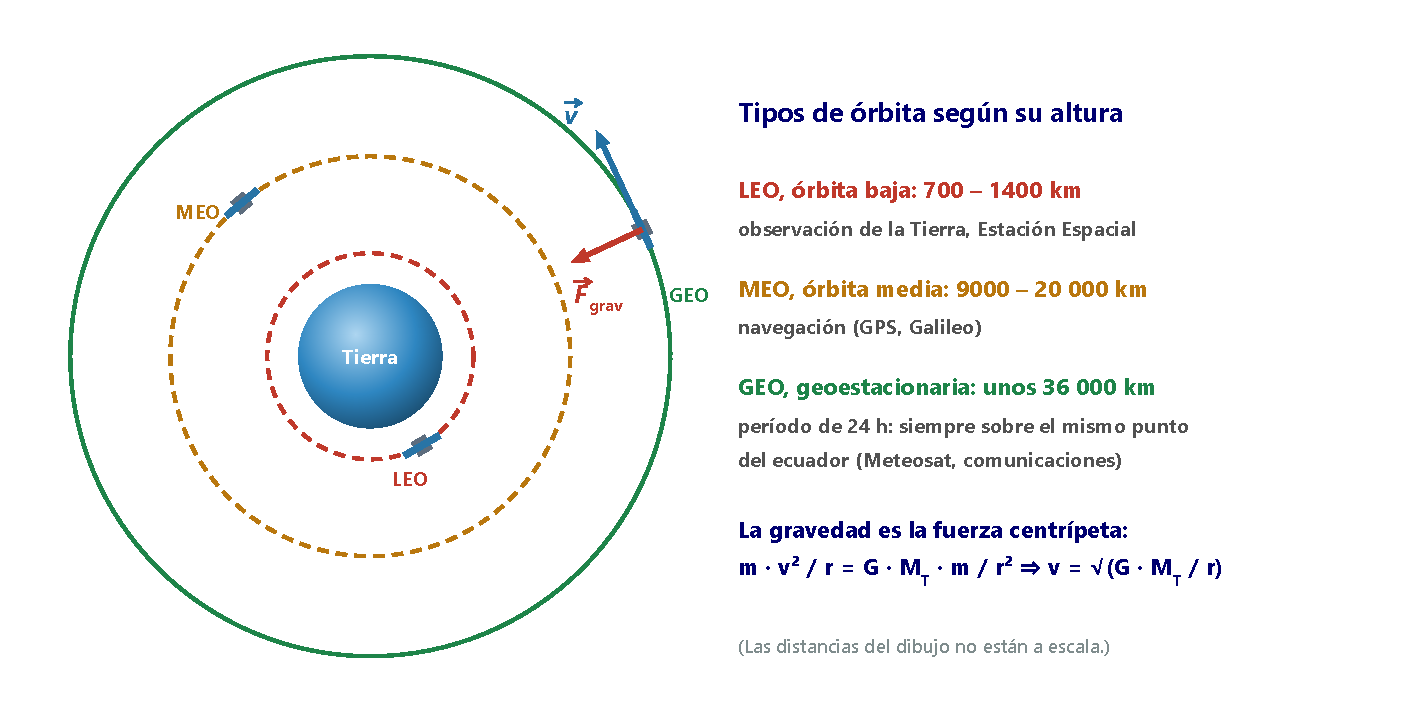
\includegraphics[width=0.95\textwidth]{images/UD9/orbitas_satelites}
    \caption{Tipos de órbita de los satélites artificiales.}
    \label{fig:orbitas_satelites}
\end{figure}

Como la Luna, un satélite está en órbita porque la atracción gravitatoria de la Tierra hace de fuerza centrípeta:
\[ m \cdot \frac{v^2}{r} = G \cdot \frac{M_T \cdot m}{r^2} \quad\Rightarrow\quad \boxed{v = \sqrt{G \cdot \frac{M_T}{r}}} \]
La velocidad orbital no depende de la masa del satélite, solo de la distancia \(r\) al centro de la Tierra: cuanto más lejos, más despacio. Y como \(v = 2\pi r / T\):
\[ \frac{4\pi^2 r^2}{T^2} = G \cdot \frac{M_T}{r} \quad\Rightarrow\quad \frac{T^2}{r^3} = \frac{4\pi^2}{G \cdot M_T} \quad\Rightarrow\quad T = \sqrt{\frac{4\pi^2 r^3}{G \cdot M_T}} \]
¡Es la tercera ley de Kepler! El cociente \(T^2/r^3\) es el mismo para todos los satélites de la Tierra. Newton demostró así que las leyes de Kepler son una consecuencia de la gravitación.

\begin{remark}
    \textbf{Basura espacial.} Se llama así a cualquier objeto artificial sin utilidad que orbita la Tierra: satélites viejos, restos de cohetes, fragmentos de choques\ldots{} Hay decenas de miles de objetos de más de \qty{10}{\cm}, cerca de un millón de fragmentos de más de \qty{1}{\cm} y miles de millones de partículas más pequeñas. A miles de kilómetros por hora, incluso un trozo pequeño puede destruir un satélite.
\end{remark}

\begin{example}
    ¿A qué velocidad gira un satélite en una órbita circular a \qty{30000}{\km} del centro de la Tierra?
    \[ v = \sqrt{G \cdot \frac{M_T}{r}} = \sqrt{\num{6.67e-11} \cdot \frac{\num{5.97e24}}{\num{3.0e7}}} = \textcolor{red}{\qty{3643}{\m\per\s}} \]
\end{example}

\begin{exercise}
    Calcula la aceleración centrípeta de un satélite que orbita a \qty{6570}{\km} del centro de la Tierra con un período de \qty{90}{\minute}.
    \begin{solu}
        \[ v = \frac{2\pi r}{T} = \frac{2\pi \cdot \num{6.57e6}}{\num{5400}} = \qty{7644}{\m\per\s} \qquad a_c = \frac{v^2}{r} = \frac{7644^2}{\num{6.57e6}} = \textcolor{red}{\qty{8.9}{\m\per\square\s}} \]
        Coincide con el valor de \(g\) a esa distancia: la aceleración centrípeta del satélite es la aceleración de la gravedad.
    \end{solu}
\end{exercise}

\begin{exercise}
    Calcula la velocidad de un satélite en una órbita circular a \qty{10000}{\km} del centro de la Tierra.
    \begin{solu}
        \[ v = \sqrt{G \cdot \frac{M_T}{r}} = \sqrt{\num{6.67e-11} \cdot \frac{\num{5.97e24}}{\num{1.0e7}}} = \textcolor{red}{\qty{6310}{\m\per\s}} \]
    \end{solu}
\end{exercise}

\subsection*{Actividades de consolidación: la síntesis newtoniana}

En estas actividades usa \(G = \qty{6.67e-11}{\newton\square\m\per\square\kg}\), \(M_T = \qty{5.97e24}{\kg}\) y \(R_T = \qty{6.37e6}{\m}\).

\begin{exercise}
    Calcula la aceleración de la gravedad a una altura sobre la superficie terrestre igual al radio de la Tierra.
    \begin{solu}
        La distancia al centro es \(2R_T = \qty{1.274e7}{\m}\):
        \[ g = \num{6.67e-11} \cdot \frac{\num{5.97e24}}{(\num{1.274e7})^2} = \textcolor{red}{\qty{2.45}{\m\per\square\s}} \]
        Al doblar la distancia al centro, \(g\) se divide entre cuatro.
    \end{solu}
\end{exercise}

\begin{exercise}
    ¿Cuánto pesa en la Luna (\(g_L = \qty{1.6}{\m\per\square\s}\)) una persona de \qty{80}{\kg}? ¿Y una piedra de \qty{1}{\kg}?
    \begin{solu}
        \(P = m \cdot g_L\): persona, \(80 \cdot \num{1.6} = \textcolor{red}{\qty{128}{\newton}}\); piedra, \(1 \cdot \num{1.6} = \textcolor{red}{\qty{1.6}{\newton}}\).
    \end{solu}
\end{exercise}

\begin{exercise}
    ¿A qué altura sobre la superficie terrestre se reduce \(g\) a la mitad?
    \begin{solu}
        \[ G \frac{M_T}{(R_T + h)^2} = \frac{1}{2} \cdot G \frac{M_T}{R_T^2} \quad\Rightarrow\quad (R_T + h)^2 = 2R_T^2 \quad\Rightarrow\quad h = (\sqrt{2} - 1) \cdot R_T = \textcolor{red}{\qty{2.64e6}{\m}} \]
        Unos \qty{2640}{\km}.
    \end{solu}
\end{exercise}

\begin{exercise}
    Calcula la velocidad de la Luna en su órbita y su período, sabiendo que está a \qty{380000}{\km} de la Tierra.
    \begin{solu}
        \[ v = \sqrt{G \frac{M_T}{r}} = \sqrt{\num{6.67e-11} \cdot \frac{\num{5.97e24}}{\num{3.8e8}}} = \textcolor{red}{\qty{1024}{\m\per\s}} \qquad T = \frac{2\pi r}{v} = \frac{2\pi \cdot \num{3.8e8}}{1024} = \textcolor{red}{\qty{2.33e6}{\s}} \]
        Unos 27 días.
    \end{solu}
\end{exercise}

\begin{exercise}
    Calcula a qué altura sobre la superficie y a qué velocidad orbita un satélite geoestacionario.
    \begin{solu}
        Un satélite geoestacionario gira en el plano del ecuador con un período de \(T = \qty{24}{\hour} = \qty{86400}{\s}\). De la expresión de la tercera ley:
        \[ r = \sqrt[3]{\frac{G \cdot M_T \cdot T^2}{4\pi^2}} = \sqrt[3]{\frac{\num{6.67e-11} \cdot \num{5.97e24} \cdot 86400^2}{4\pi^2}} = \qty{4.22e7}{\m} \]
        \[ h = r - R_T = \num{4.22e7} - \num{6.37e6} = \textcolor{red}{\qty{3.59e7}{\m}} \ (\text{unos } \qty{35900}{\km}) \qquad v = \sqrt{G \frac{M_T}{r}} = \textcolor{red}{\qty{3071}{\m\per\s}} \]
    \end{solu}
\end{exercise}

\begin{exercise}
    Calcula la velocidad, el período y la aceleración centrípeta de un satélite en órbita circular a \qty{2000}{\km} de altura.
    \begin{solu}
        \(r = \num{6.37e6} + \num{2.0e6} = \qty{8.37e6}{\m}\).
        \[ v = \sqrt{\num{6.67e-11} \cdot \frac{\num{5.97e24}}{\num{8.37e6}}} = \textcolor{red}{\qty{6897}{\m\per\s}} \qquad T = \frac{2\pi r}{v} = \textcolor{red}{\qty{7625}{\s}} \qquad a_c = \frac{v^2}{r} = \textcolor{red}{\qty{5.68}{\m\per\square\s}} \]
    \end{solu}
\end{exercise}

\begin{exercise}
    La masa de Júpiter es unas 318 veces la de la Tierra y su radio, unas 11 veces mayor. Calcula la gravedad en Júpiter (\(g_T = \qty{9.8}{\m\per\square\s}\)).
    \begin{solu}
        Dividimos las expresiones de \(g\) de los dos planetas; \(G\) se simplifica:
        \[ \frac{g_J}{g_T} = \frac{M_J}{M_T} \cdot \left(\frac{R_T}{R_J}\right)^2 = 318 \cdot \frac{1}{11^2} = \num{2.63} \quad\Rightarrow\quad g_J = \num{2.63} \cdot \num{9.8} = \textcolor{red}{\qty{25.8}{\m\per\square\s}} \]
    \end{solu}
\end{exercise}

\begin{exercise}
    ¿Cuánto vale la gravedad en un planeta con el mismo radio que la Tierra y la mitad de masa?
    \begin{solu}
        \(g\) es proporcional a la masa: \(g = \dfrac{\num{9.8}}{2} = \textcolor{red}{\qty{4.9}{\m\per\square\s}}\).
    \end{solu}
\end{exercise}

\begin{exercise}
    Calcula la gravedad en la superficie de Plutón, cuya masa es \qty{1.25e22}{\kg} y su radio, \qty{1188.3}{\km}.
    \begin{solu}
        \[ g = \num{6.67e-11} \cdot \frac{\num{1.25e22}}{(\num{1.1883e6})^2} = \textcolor{red}{\qty{0.59}{\m\per\square\s}} \]
    \end{solu}
\end{exercise}

%========================================================================================
\section[La fuerza eléctrica]{La fuerza eléctrica: una fuerza de la naturaleza}
%========================================================================================

Hasta comienzos del siglo \textsc{xx}, con el descubrimiento del electrón y los primeros modelos atómicos, no se explicó la naturaleza eléctrica de la materia. Los átomos tienen un núcleo con carga positiva (los protones) y, a su alrededor, electrones con carga negativa. Normalmente hay tantos protones como electrones y el átomo es \textbf{neutro}. Pero los electrones más externos pueden pasar de un cuerpo a otro: el cuerpo que \textbf{gana electrones} queda con carga \textbf{negativa}, y el que los \textbf{pierde}, con carga \textbf{positiva} (figura~\ref{fig:cargas_electricas}).

\begin{remark}
    En el siglo \textsc{xviii}, Benjamin Franklin demostró con su famosa cometa que los rayos son grandes descargas eléctricas. Como las descargas se dirigen hacia los objetos puntiagudos, inventó el \textbf{pararrayos}, que ha evitado muchas desgracias.
\end{remark}

\subsection{Unidades de la carga eléctrica}

La carga del electrón es la unidad natural de carga: la carga de cualquier cuerpo es siempre un \textbf{múltiplo entero} de ella. Como es muy pequeña, en el SI la carga, \(Q\), se mide en \textbf{culombios} (\unit{\coulomb}):
\[ e = \qty{1.6e-19}{\coulomb} \qquad\qquad \qty{1}{\coulomb} = \num{6.25e18}~\text{electrones} \]
En la práctica se usan submúltiplos como el microculombio: \(\qty{1}{\micro\coulomb} = \qty{1e-6}{\coulomb}\).

\subsection{Fuerzas entre cargas eléctricas. Ley de Coulomb}

\begin{figure}[H]
    \centering
    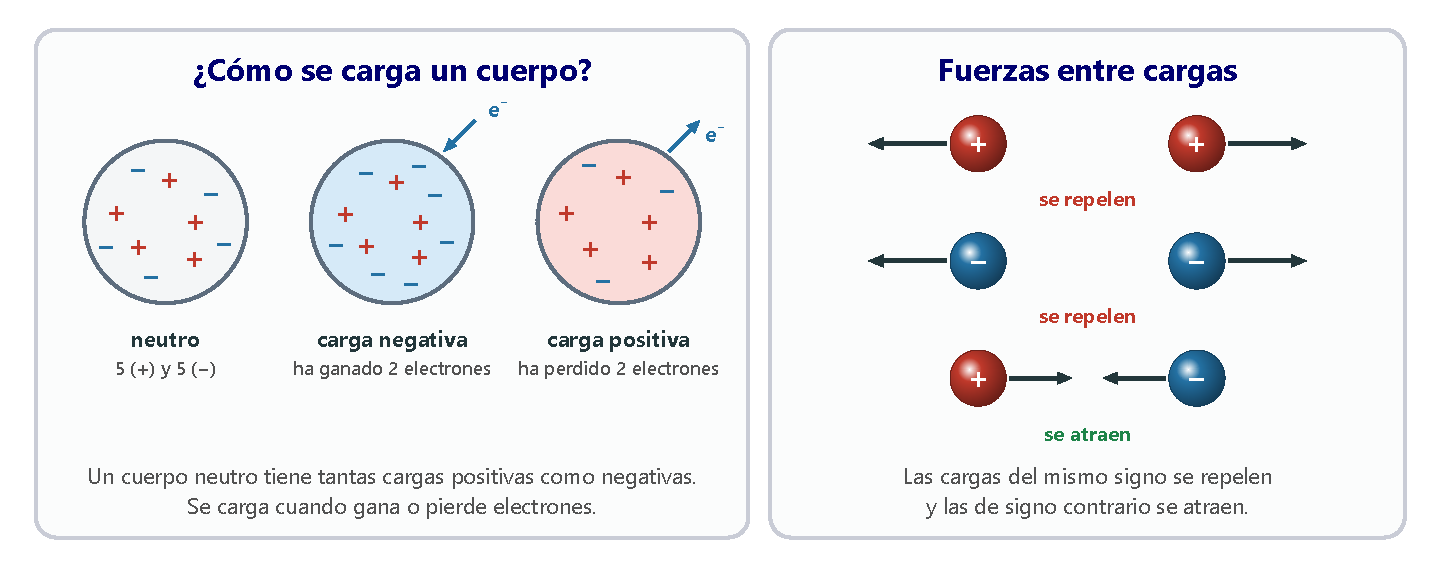
\includegraphics[width=\textwidth]{images/UD9/cargas_electricas}
    \caption{Cómo se carga un cuerpo y cómo actúan las fuerzas entre cargas.}
    \label{fig:cargas_electricas}
\end{figure}

En 1785, Charles-Augustin de \textbf{Coulomb} midió con una balanza de torsión las fuerzas entre cuerpos cargados. Las cargas del \textbf{mismo signo se repelen} y las de \textbf{signo contrario se atraen}, y el valor de la fuerza lo da la \textbf{ley de Coulomb}:

\begin{definition}[Ley de Coulomb]
    La fuerza con que se atraen o se repelen dos cargas puntuales \(Q\) y \(Q'\) es directamente proporcional al producto de sus valores e inversamente proporcional al cuadrado de la distancia \(r\) que las separa:
    \[ F = k \cdot \frac{Q \cdot Q'}{r^2} \qquad\qquad k = \qty{9e9}{\newton\square\m\per\square\coulomb} \ (\text{en el vacío o el aire}) \]
\end{definition}

Fíjate en el parecido con la ley de gravitación universal. Pero hay dos diferencias importantes: la fuerza eléctrica puede ser de \textbf{atracción o de repulsión}, y es \textbf{muchísimo más intensa}.

\begin{example}
    En un átomo de hidrógeno, el protón y el electrón están a \qty{5e-11}{\m}. Compara la fuerza eléctrica y la gravitatoria entre ellos (\(e = \qty{1.6e-19}{\coulomb}\), \(m_p = \qty{1.67e-27}{\kg}\), \(m_e = \qty{9.1e-31}{\kg}\)).
    \[ F_e = \num{9e9} \cdot \frac{(\num{1.6e-19})^2}{(\num{5e-11})^2} = \textcolor{red}{\qty{9.2e-8}{\newton}} \]
    \[ F_g = \num{6.67e-11} \cdot \frac{\num{1.67e-27} \cdot \num{9.1e-31}}{(\num{5e-11})^2} = \textcolor{red}{\qty{4.1e-47}{\newton}} \]
    La fuerza eléctrica es unas \(10^{39}\) veces mayor: dentro del átomo, la gravedad no cuenta.
\end{example}

\begin{exercise}
    ¿Puede existir un cuerpo cuya carga sea una fracción de la carga del electrón?
    \begin{solu}
        \textcolor{red}{No}. La carga del electrón es la unidad elemental: la carga de cualquier cuerpo es un número entero de veces esa carga.
    \end{solu}
\end{exercise}

\begin{exercise}
    Los dos protones del núcleo de helio están separados unos \qty{1e-15}{\m}. Calcula la fuerza eléctrica de repulsión entre ellos.
    \begin{solu}
        \[ F = k \cdot \frac{Q \cdot Q'}{r^2} = \num{9e9} \cdot \frac{(\num{1.6e-19})^2}{(\num{1e-15})^2} = \textcolor{red}{\qty{230}{\newton}} \]
        Es una fuerza enorme para dos partículas tan pequeñas: los protones se mantienen juntos gracias a otra fuerza todavía más intensa, la fuerza nuclear fuerte.
    \end{solu}
\end{exercise}

\subsection{El potencial eléctrico}

Imagina una carga positiva \(Q\) fija. Si queremos acercarle otra carga positiva, tenemos que vencer la repulsión, es decir, realizar un trabajo. Ese trabajo no se pierde: queda almacenado como \textbf{energía potencial electrostática}, \(E_p\).

\begin{definition}[Potencial eléctrico]
    El \textbf{potencial eléctrico}, \(V\), en un punto es la energía potencial que adquiere la unidad de carga positiva al traerla desde el infinito hasta ese punto. Es una magnitud escalar. A una distancia \(r\) de una carga \(Q\):
    \[ V = \frac{E_p}{q} = k \cdot \frac{Q}{r} \]
    Su unidad es el \textbf{voltio} (\unit{\volt}): \(\qty{1}{\volt} = \dfrac{\qty{1}{\joule}}{\qty{1}{\coulomb}}\).
\end{definition}

\subsection{Diferencia de potencial entre dos puntos}

Si en el punto A el potencial es \(V_A\) y en el punto B es \(V_B\), la \textbf{diferencia de potencial} entre ellos es \(V_A - V_B\), y también se mide en voltios. El trabajo que hay que realizar para llevar una carga \(q\) de A a B es:
\[ W_{A \to B} = q \cdot (V_B - V_A) \]
Si sale negativo, no hace falta hacer trabajo: la propia fuerza eléctrica lleva la carga de A a B.

\begin{example}
    Una carga \(Q = \qty{1}{\micro\coulomb}\) está en un punto O. Los puntos A y B están alineados con ella, a \qty{3}{\m} y \qty{6}{\m}. Calcula: a) el potencial en A y en B; b) el trabajo para llevar una carga de \qty{0.1}{\micro\coulomb} de A a B.

    a) \(V_A = k \dfrac{Q}{r_A} = \num{9e9} \cdot \dfrac{\num{1e-6}}{3} = \textcolor{red}{\qty{3000}{\volt}}\); \quad \(V_B = \num{9e9} \cdot \dfrac{\num{1e-6}}{6} = \textcolor{red}{\qty{1500}{\volt}}\)

    b) \(W = q \cdot (V_B - V_A) = \num{1e-7} \cdot (1500 - 3000) = \textcolor{red}{\qty{-1.5e-4}{\joule}}\). El signo negativo indica que la carga se aleja \textbf{sola}, empujada por la repulsión de \(Q\).
\end{example}

\begin{exercise}
    Una tormenta es una manifestación de las fuerzas eléctricas. Busca información sobre cómo se distribuyen las cargas en las nubes para que se formen los rayos.
    \begin{solu}
        Respuesta libre. Dentro de las nubes de tormenta, los choques entre cristales de hielo y gotas separan las cargas: la parte \textcolor{red}{superior} de la nube queda con carga \textcolor{red}{positiva} y la \textcolor{red}{inferior}, con carga \textcolor{red}{negativa}, que a su vez induce carga positiva en el suelo. Cuando la diferencia de potencial es enorme, el aire deja pasar una descarga: el \textbf{rayo}. El \textbf{relámpago} es su luz y el \textbf{trueno}, su sonido.
    \end{solu}
\end{exercise}

\subsection*{Actividades de consolidación: la fuerza eléctrica}

En estas actividades usa \(k = \qty{9e9}{\newton\square\m\per\square\coulomb}\).

\begin{exercise}
    Dos cuerpos con cargas de \qty{2.5}{\micro\coulomb} y \qty{3}{\micro\coulomb}, del mismo signo, están a \qty{5}{\cm}. ¿Se atraen o se repelen? ¿Con qué fuerza se atraerían si sus cargas fueran de signo contrario?
    \begin{solu}
        Como tienen el mismo signo, \textcolor{red}{se repelen}. Si fueran de signo contrario se atraerían con una fuerza del mismo módulo:
        \[ F = \num{9e9} \cdot \frac{\num{2.5e-6} \cdot \num{3e-6}}{(\num{0.05})^2} = \textcolor{red}{\qty{27}{\newton}} \]
    \end{solu}
\end{exercise}

\begin{exercise}
    ¿Cuál es el potencial en un punto si una carga de \qty{1}{\micro\coulomb} colocada en él tiene una energía potencial de \qty{0.001}{\joule}?
    \begin{solu}
        \(V = \dfrac{E_p}{q} = \dfrac{\num{0.001}}{\num{1e-6}} = \textcolor{red}{\qty{1000}{\volt}}\).
    \end{solu}
\end{exercise}

\begin{exercise}
    El potencial en un punto A es \qty{125}{\volt} y en un punto B, \qty{200}{\volt}. ¿Qué trabajo hay que realizar para llevar una carga de \qty{1}{\micro\coulomb} de A a B?
    \begin{solu}
        \(W = q \cdot (V_B - V_A) = \num{1e-6} \cdot (200 - 125) = \textcolor{red}{\qty{7.5e-5}{\joule}}\).
    \end{solu}
\end{exercise}

\begin{exercise}
    Una carga \(Q = \qty{2}{\micro\coulomb}\) está en un punto P. Los puntos A y B están alineados con ella, a \qty{2}{\m} y \qty{5}{\m}. Calcula:
    \begin{enumerate}[label=\alph*)]
        \item El potencial que crea \(Q\) en A y en B.
        \item El trabajo necesario para llevar una carga de \qty{-0.1}{\micro\coulomb} de A a B.
    \end{enumerate}
    \begin{solu}
        a) \(V_A = \num{9e9} \cdot \dfrac{\num{2e-6}}{2} = \textcolor{red}{\qty{9000}{\volt}}\); \(V_B = \num{9e9} \cdot \dfrac{\num{2e-6}}{5} = \textcolor{red}{\qty{3600}{\volt}}\).
        b) \(W = q \cdot (V_B - V_A) = (\num{-1e-7}) \cdot (3600 - 9000) = \textcolor{red}{\qty{5.4e-4}{\joule}}\). Es positivo: hay que hacer trabajo para alejar la carga negativa, porque \(Q\) la atrae.
    \end{solu}
\end{exercise}

%========================================================================================
\section[La fuerza magnética]{La fuerza magnética: una fuerza de la naturaleza}
%========================================================================================

La \textbf{magnetita} es un mineral que atrae el hierro, el cobalto, el níquel y algunas aleaciones de estos metales. Esta propiedad se llama \textbf{magnetismo}, y los cuerpos que la tienen son \textbf{imanes}.

\subsection{Clasificación de los imanes}

\begin{itemize}
    \item \textbf{Naturales y artificiales.} Un trozo de magnetita es un imán natural; un trozo de hierro o de acero imantado es un imán artificial.
    \item \textbf{Permanentes y temporales.} Si se ponen en contacto con un imán un trozo de hierro y uno de acero, los dos se imantan. Al separarlos, el acero sigue siendo un imán (\textbf{imán permanente}), pero el hierro deja de serlo (\textbf{imán temporal}).
\end{itemize}

\subsection{Propiedades de los imanes}

\begin{figure}[H]
    \centering
    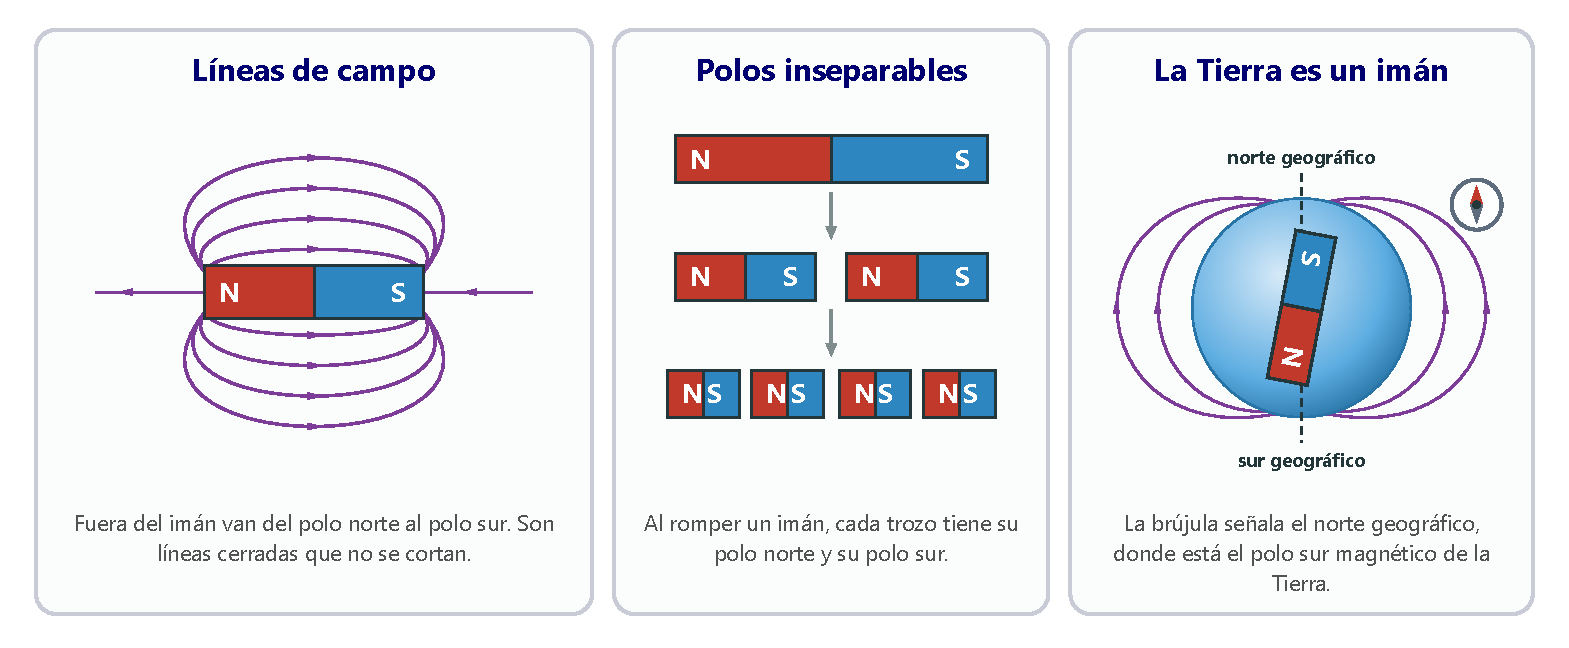
\includegraphics[width=\textwidth]{images/UD9/imanes}
    \caption{Líneas de campo de un imán de barra, imán roto y la Tierra como gran imán.}
    \label{fig:imanes}
\end{figure}

\begin{itemize}
    \item El magnetismo es más intenso en los extremos del imán, sus \textbf{polos}: el \textbf{polo norte} y el \textbf{polo sur}.
    \item \textbf{No se puede aislar un polo}: si rompemos un imán, cada trozo tiene su polo norte y su polo sur.
    \item Los polos del mismo nombre se \textbf{repelen} y los de distinto nombre se \textbf{atraen}.
\end{itemize}

Una \textbf{brújula} es una aguja imantada que gira libremente; uno de sus extremos se orienta hacia el norte geográfico. Por eso decimos que la Tierra es un gigantesco imán natural cuyo \textbf{polo sur magnético está cerca del polo norte geográfico} (el polo norte de la aguja es atraído por un polo sur). En realidad, el polo magnético está a unos \qty{1600}{\km} del polo geográfico, en el norte de Canadá, y se va desplazando con los años.

\paragraph{¿Qué son las líneas de campo magnético?} Si ponemos un papel sobre un imán y espolvoreamos limaduras de hierro, estas se ordenan formando unas líneas: las \textbf{líneas de campo magnético}. Son líneas \textbf{cerradas} que \textbf{no se cortan}; fuera del imán van del polo norte al polo sur, y por dentro, del sur al norte (figura~\ref{fig:imanes}).

\begin{marker}
    \textbf{Las auroras polares.} El Sol emite continuamente partículas con carga eléctrica (el \emph{viento solar}). El campo magnético terrestre las desvía y las conduce hacia las regiones polares. Allí chocan con los gases de la atmósfera, que emiten luz de colores: el oxígeno produce los tonos verdes y rojos, y el nitrógeno, los azules y violetas.
\end{marker}

\begin{exercise}
    Distingue entre imán temporal e imán permanente y entre imán natural e imán artificial.
    \begin{solu}
        Un imán \textcolor{red}{permanente} conserva la imantación mucho tiempo (por ejemplo, el acero); uno \textcolor{red}{temporal} solo es un imán mientras está en contacto con otro imán (por ejemplo, el hierro dulce). Un imán \textcolor{red}{natural} es un mineral que ya es magnético, como la magnetita; uno \textcolor{red}{artificial} es un material al que se ha imantado.
    \end{solu}
\end{exercise}

\begin{exercise}
    Explica por qué las auroras polares son un fenómeno magnético.
    \begin{solu}
        Las partículas cargadas del viento solar son \textcolor{red}{desviadas por el campo magnético terrestre}, que las guía hacia los polos siguiendo sus líneas de campo. Por eso las auroras solo se ven en las zonas cercanas a los polos, donde esas partículas chocan con los gases de la atmósfera y los hacen emitir luz.
    \end{solu}
\end{exercise}

%========================================================================================
\section[El electromagnetismo]{¿Qué relación hay entre electricidad y magnetismo? El electromagnetismo}
%========================================================================================

Durante siglos se pensó que electricidad y magnetismo eran fenómenos distintos. Dos experiencias del siglo \textsc{xix} demostraron que están íntimamente relacionados (figura~\ref{fig:oersted_faraday}).

\begin{figure}[H]
    \centering
    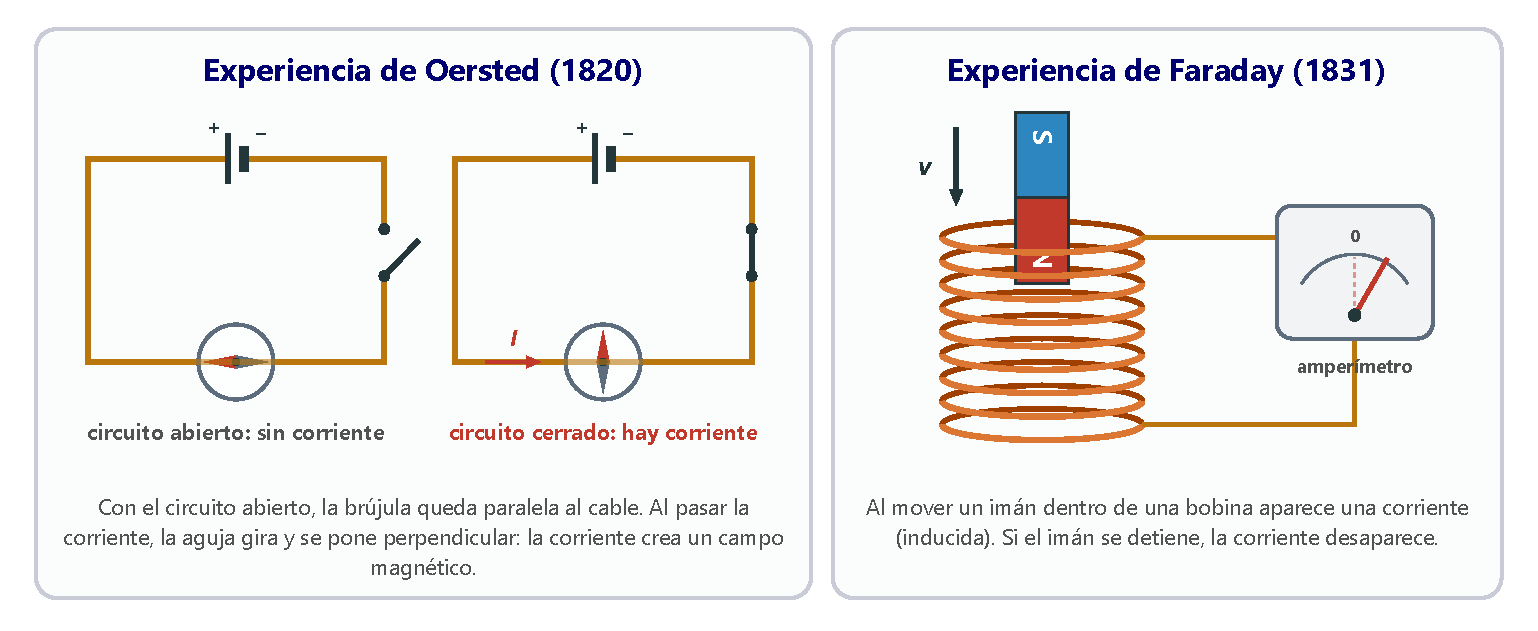
\includegraphics[width=\textwidth]{images/UD9/oersted_faraday}
    \caption{Las experiencias de Oersted y de Faraday.}
    \label{fig:oersted_faraday}
\end{figure}

\paragraph{La experiencia de Oersted.} En 1820, \textbf{Hans Christian Oersted} descubrió por casualidad que una corriente eléctrica desvía una brújula. Con el circuito abierto, la brújula situada bajo el cable se orienta de forma natural, paralela a él. Al cerrar el circuito, la aguja gira hasta ponerse perpendicular al cable, y si se invierte el sentido de la corriente, gira en sentido contrario. Conclusiones:
\begin{itemize}
    \item Una \textbf{carga eléctrica en reposo} solo produce fenómenos electrostáticos.
    \item Una \textbf{carga en movimiento} (una corriente) produce además un \textbf{campo magnético} a su alrededor.
\end{itemize}

\paragraph{La experiencia de Faraday.} En 1831, \textbf{Michael Faraday} comprobó lo contrario: un imán puede producir corriente eléctrica. Conectó una bobina a un medidor de corriente y observó que:
\begin{itemize}
    \item Al introducir un imán en la bobina, aparece una corriente; al sacarlo, aparece una corriente de sentido contrario.
    \item Si el imán está quieto dentro de la bobina, \textbf{no hay corriente}.
    \item Si se acerca el otro polo del imán, la corriente cambia de sentido.
\end{itemize}

\begin{definition}[Corriente inducida]
    Un \textbf{campo magnético variable} produce una corriente eléctrica en un circuito cercano, llamada \textbf{corriente inducida}. Existe mientras el campo magnético varía y es tanto mayor cuanto más rápida es la variación.
\end{definition}

En este fenómeno, la \textbf{inducción electromagnética}, se basan los generadores de las centrales eléctricas, las dinamos y las cocinas de inducción; y en el efecto descubierto por Oersted, los electroimanes y los motores eléctricos.

\begin{exercise}
    Describe las experiencias de Oersted y de Faraday. Ayúdate de esquemas o dibujos.
    \begin{solu}
        Respuesta libre basada en la figura~\ref{fig:oersted_faraday}. \textcolor{red}{Oersted}: una corriente eléctrica desvía una brújula, es decir, \textcolor{red}{la corriente crea un campo magnético}. \textcolor{red}{Faraday}: al mover un imán dentro de una bobina aparece una corriente, es decir, \textcolor{red}{un campo magnético variable crea una corriente eléctrica}.
    \end{solu}
\end{exercise}
